\documentclass[a4paper,oneside,12pt]{book}
%% === nezbytné balíčky:
\usepackage[T1]{fontenc}    % kódování písma
%\usepackage[IL2]{fontenc}  % kódování písma
\usepackage{graphicx}
\usepackage[utf8]{inputenc}     % vstupní znaková sada tohoto dokumentu: UTF-8
%\usepackage[cp1250]{inputenc}  % vstupní znaková sada tohoto dokumentu: Windows 1250
%\usepackage[latin2]{inputenc}  % vstupní znaková sada tohoto dokumentu: ISO Latin 2

\usepackage{algpseudocode}

\usepackage{siunitx}
\usepackage[czech]{babel} % česky psaná práce, typografická pravidla. 
\usepackage{amsmath}
\usepackage{listings}
\usepackage{listings}
\usepackage{xcolor}

\definecolor{codegray}{rgb}{0.5,0.5,0.5}
\definecolor{codeblue}{rgb}{0,0,1}
\definecolor{codegreen}{rgb}{0,0.6,0}

\lstdefinelanguage{yaml}{
  morekeywords={true,false,null,yes,no,code,keywords,land_use, URL,buffer_layers,input_layer_name,controlling_atr_name,buffer_levels,priority,values,distance,default_buffer, layers, name,base_use_code,controlling_attribute,value_increments, N, J, L, S, layer_name},
  sensitive=false,
  morecomment=[l]{\#},
  morestring=[b]",
  morestring=[b]',
  alsoletter={:\-},       
  moredelim=[s][\color{codeblue}]{:}{\ },
  moredelim=[l][\color{codegray}]{\#}
}

\lstdefinestyle{myyaml}{
    language=yaml,
    basicstyle=\ttfamily\footnotesize,
    keywordstyle=\color{codeblue}\bfseries,
    commentstyle=\color{codegray},
    stringstyle=\color{codegreen},
    breaklines=true,
    numbers=left,
    numberstyle=\tiny\color{codegray},
    frame=single
}

\lstset{
  inputencoding=utf8,
  extendedchars=true,
  literate={á}{{\'a}}1 {č}{{\v{c}}}1 {ď}{{\v{d}}}1 {é}{{\'e}}1
           {ě}{{\v{e}}}1 {í}{{\'i}}1 {ň}{{\v{n}}}1 {ó}{{\'o}}1
           {ř}{{\v{r}}}1 {š}{{\v{s}}}1 {ť}{{\v{t}}}1 {ú}{{\'u}}1
           {ů}{{\r{u}}}1 {ý}{{\'y}}1 {ž}{{\v{z}}}1
           {Á}{{\'A}}1 {Č}{{\v{C}}}1 {Ď}{{\v{D}}}1 {É}{{\'E}}1
           {Ě}{{\v{E}}}1 {Í}{{\'I}}1 {Ň}{{\v{N}}}1 {Ó}{{\'O}}1
           {Ř}{{\v{R}}}1 {Š}{{\v{S}}}1 {Ť}{{\v{T}}}1 {Ú}{{\'U}}1
           {Ů}{{\r{U}}}1 {Ý}{{\'Y}}1 {Ž}{{\v{Z}}}1,
  style=myyaml
}

\lstdefinestyle{mypython}{
    language=Python,
    basicstyle=\ttfamily\footnotesize,
    keywordstyle=\color{codeblue}\bfseries,
    commentstyle=\color{codegray},
    stringstyle=\color{codegreen},
    breaklines=true,
    numbers=left,
    numberstyle=\tiny\color{codegray},
    frame=single
}
\lstset{
  inputencoding=utf8,
  extendedchars=true,
  literate={á}{{\'a}}1 {č}{{\v{c}}}1 {ď}{{\v{d}}}1 {é}{{\'e}}1
           {ě}{{\v{e}}}1 {í}{{\'i}}1 {ň}{{\v{n}}}1 {ó}{{\'o}}1
           {ř}{{\v{r}}}1 {š}{{\v{s}}}1 {ť}{{\v{t}}}1 {ú}{{\'u}}1
           {ů}{{\r{u}}}1 {ý}{{\'y}}1 {ž}{{\v{z}}}1
           {Á}{{\'A}}1 {Č}{{\v{C}}}1 {Ď}{{\v{D}}}1 {É}{{\'E}}1
           {Ě}{{\v{E}}}1 {Í}{{\'I}}1 {Ň}{{\v{N}}}1 {Ó}{{\'O}}1
           {Ř}{{\v{R}}}1 {Š}{{\v{S}}}1 {Ť}{{\v{T}}}1 {Ú}{{\'U}}1
           {Ů}{{\r{U}}}1 {Ý}{{\'Y}}1 {Ž}{{\v{Z}}}1,
  style=mypython
}
\lstdefinestyle{mypseudocode}{
    language=[LaTeX]TeX,
    morekeywords={Pokud,Jinak,Opakuj,Až,Pro,Ve,Od,Do,Krok,Def,Pak,Return,POKUD,JINAK,KONEC,PODMINKY,VRATIT, A , OPAKUJ, PRO, V, CYKLU, KAZDY, NEUSPECH, USPECH, NEBO, POKRACUJ},
    keywordstyle=\color{codeblue}\bfseries,
    commentstyle=\color{codegray}\itshape,
    stringstyle=\color{codegreen},
    basicstyle=\ttfamily\footnotesize,
    breaklines=true,
    numbers=left,
    numberstyle=\tiny\color{codegray},
    frame=single,
    inputencoding=utf8,
    extendedchars=true,
    mathescape=true,                
    literate={á}{{\'a}}1 {č}{{\v{c}}}1 {ď}{{\v{d}}}1 {é}{{\'e}}1
             {ě}{{\v{e}}}1 {í}{{\'i}}1 {ň}{{\v{n}}}1 {ó}{{\'o}}1
             {ř}{{\v{r}}}1 {š}{{\v{s}}}1 {ť}{{\v{t}}}1 {ú}{{\'u}}1
             {ů}{{\r{u}}}1 {ý}{{\'y}}1 {ž}{{\v{z}}}1
             {Á}{{\'A}}1 {Č}{{\v{C}}}1 {Ď}{{\v{D}}}1 {É}{{\'E}}1
             {Ě}{{\v{E}}}1 {Í}{{\'I}}1 {Ň}{{\v{N}}}1 {Ó}{{\'O}}1
             {Ř}{{\v{R}}}1 {Š}{{\v{S}}}1 {Ť}{{\v{T}}}1 {Ú}{{\'U}}1
             {Ů}{{\r{U}}}1 {Ý}{{\'Y}}1 {Ž}{{\v{Z}}}1 {@}{{{$\leftarrow$}}}1
}
\lstset{style=mypseudocode}

%Překládejte pomocí "latex.exe" nebo "pdflatex.exe"
%\usepackage{czech} % česky psaná práce. Překládejte pomocí "pdfCSlatex.exe" ("cslatex.exe" asi bude mít problém s balíkem geometry)
\usepackage{hhline} % Add the hhline package
\usepackage[a4paper, hmarginratio=3:2]{geometry} % využití A4 stránky a nastavení okrajů (u vazby bude širší)
\usepackage{afterpage}
\usepackage{caption}
\usepackage{pdfpages} % pokud nemáte formulář "Zadání bak./dipl. práce" naskenovaný jako PDF, tak ZAKOMENTUJTE
\usepackage[hidelinks]{hyperref} % v PDF budou klikací odkazy ("hidelinks" je nebude rámovat)
%% === balíčky, které se mohou hodit:
%\usepackage{encxvlna} % postará se o spojky a předložky, které dle českých pravidel nesmí být na konci řádku. Dokumentace: http://texdoc.net/texmf-dist/doc/generic/encxvlna/encxvlna.pdf (chová se správně k "vnitřku" listings?)

\usepackage{graphicx} % balíček pro vkládání rastrových grafických souborů (PNG apod.)
%\usepackage{epsfig} % balíčky pro vkládání grafických souborů typu EPS
\usepackage{float} % rozšířené možnosti umístění obrázků

%\usepackage{caption} % pro popisky obrázků, tabulek atd.

\usepackage{tabularx} % rozšířené možnosti tabulek
%\usepackage{tabu} % jiný balík pro rozšířené možnosti tabulek

\usepackage{listings}  % balíček vhodný pro ukázky zdrojového kódu v~textu práce/příloh. Nutno nastavit! http://ftp.cvut.cz/tex-archive/macros/latex/contrib/listings/listings.pdf
\usepackage{amsmath} % balíček pro pokročilou matematickou sazbu
%\usepackage{color} % pro možnost barevného textu
%\usepackage{fancybox} % umožňuje pokročilé rámečkování

%\usepackage{index} % nutno použít v případě tvorby rejstříku balíčkem makeindex
%\newindex{default}{idx}{ind}{Rejstřík} % zavádí rejstřík v případě použití balíku index

% Wrapper for Python listings
\lstnewenvironment{pythoncode}[1][]{
  \renewcommand{\lstlistingname}{Kód}% 〈Czech “Code”〉
  \lstset{style=mypython,#1}
}{}

% Wrapper for Pseudocode listings
\lstnewenvironment{pseudocode}[1][]{
  \renewcommand{\lstlistingname}{Pseudokód}% 〈Czech “Pseudocode”〉
  \lstset{style=mypseudocode,#1}
}{}

\frenchspacing % za větou bude mezislovní mezera (v anglických textech je mezera za větou delší)
\widowpenalty=1000 % "síla" zákazu vdov (= jeden řádek ze začátku odstavce na konci stránky)
\clubpenalty=1000 % "síla" zákazu sirotků (= jeden řádek/slovo z konce odstavce samostatně na začátku stránky)
\brokenpenalty=1000 % "síla" zákazu zlomu stránky za řádkem, který má na konci rozdělené slovo

\topmargin=-15mm      % horní okraj trochu menší
\textwidth=150mm      % šířka textu na stránce
\textheight=240mm     % "výška" textu na stránce


\pagenumbering{arabic} % číslování stránek arabskými číslicemi
\pagestyle{plain}      % stránky číslované dole uprostřed

\parindent=0pt % odsazení 1. řádku odstavce
\parskip=7pt   % mezera mezi odstavci

\newcommand{\ti}{\textit} % zkrácený příkaz pro kurzívu
\newcommand{\tb}{\textbf} % zkrácený příkaz pro tučné písmo








%% --- zde jsou zavedeny některé "konstanty" - některé musíte změnit! --- %%
\newcommand{\cvut}{České vysoké učení technické v~Praze}
\newcommand{\fjfi}{Fakulta stavební}
\newcommand{\ksi}{Katedra geomatiky}
\newcommand{\program}{Geodézie a kartografie} % změňte, pokud máte jiný stud. program
\newcommand{\obor}{} % změňte, pokud máte jiný obor

\newcommand{\druh}{Diplomová práce} % nebo "Diplomová práce"
\newcommand{\woman}{} % pokud jste ŽENA, ZMĚŇTE na: ...{\woman}{a} (je to do Prohlášení)

\newcommand{\logoCVUT}{
\includegraphics{pictures/symbol_cvut_konturova_verze_cb.pdf}} % logo ČVUT -- podle grafického manuálu ČVUT platného od prosince 2016. Pokud nevyhovuje PDF-verze, tak použijte jinou variantu loga: https://www.cvut.cz/logo-a-graficky-manual -> "Symbol a logo ČVUT v Praze"). Pokud chcete logo úplně vynechat, zadejte místo "\includegraphics{...}" text "\vspace{35mm}"

% přesně podle formuláře "Zadání bak./dipl. práce" VYPLŇTE:
\newcommand{\nazevcz}{Vývoj zásuvného modulu QGIS pro určení využití území a potřeby analýz odtokových poměrů}    % český název práce (přesně podle zadání!)
\newcommand{\nazeven}{Development of a QGIS Plugin for Land Use Determination and Purposes of Runoff Analysis}          % anglický název práce (přesně podle zadání!)
\newcommand{\autor}{Bc. Josef Jehlička}   % vyplňte své jméno a příjmení (s akademickým titulem, máte-li jej)
\newcommand{\vedouci}{Ing. Martin Landa, Ph.D. } % vyplňte jméno a příjmení vedoucího práce, včetně titulů, např.: Doc. Ing. Ivo Malý, Ph.D.
\newcommand{\druhyvedouci}{doc. Ing. Petr Kavka, Ph.D.}
\newcommand{\pracovisteVed}{\ksi, \fjfi, \cvut} % ZMĚŇTE, pokud vedoucí Vaší práce není z KSI
\newcommand{\konzultant}{--} % POKUD MÁTE určeného konzultanta, NAPIŠTE jeho jméno a příjmení
\newcommand{\pracovisteKonz}{--} % POKUD MÁTE konzultanta, NAPIŠTE jeho pracoviště

% podle skutečnosti VYPLŇTE:
\newcommand{\rok}{2025}  % rok odevzdání práce (jen rok odevzdání, nikoli celý akademický rok!)
\newcommand{\kde}{Praze} % studenti z Děčína ZMĚNÍ na: "Děčíně" (doplní se k "prohlášení")

\newcommand{\klicova}{Klíčová slova}   % zde NAPIŠTE česky max. 5 klíčových slov
\newcommand{\keyword}{Key words}       % zde NAPIŠTE anglicky max. 5 klíčových slov (přeložte z češtiny)
\newcommand{\abstrCZ}{Popis práce česky}    % zde NAPIŠTE abstrakt v češtině (cca 7 vět, min. 80 slov)
\newcommand{\abstrEN}{Popis práce anglicky} % zde NAPIŠTE abstrakt v angličtině

\newcommand{\prohlaseni}{Prohlašuji, že jsem diplomovou práci s názvem "Vývoj QGIS zásuvného modulu pro potřeby výpočtu objemu přímého odtoku metodou SCS-CN“ vypracoval samostatně s odborným vedením pana Ing. Martina Landy, Ph.D a doc. Ing. Petra Kavky, Ph.D. Použitá literatura a další podklady, které byly použity pro tuto diplomovou práci, jsou uvedeny v seznamu literatury. Dále prohlašuji, že nemám závažný důvod proti užití tohoto školního díla ve smyslu § 60 zákona č. 121/2000 Sb., o právu autorském, o právech souvisejících s právem autorským a o změně některých zákonů.
} % text prohlášení můžete mírně upravit :-)

\newcommand{\podekovani}{Tímto bych chtěl poděkovat } % NAPIŠTE poděkování, např. svému vedoucímu:
% Děkuji Ing. Eleonoře Krtečkové, Ph.D. za vedení mé bakalářské práce a za podnětné návrhy, které ji obohatily.
% NEBO:
% Děkuji vedoucímu práce doc. Pafnutijovi Snědldítětikaši, Ph.D. za neocenitelné rady a pomoc při tvorbě bakalářské práce.














\begin{document}
%%%%%%%%%%%% TITULNÍ STRANA -- na následujících cca 30 řádků NESAHEJTE!!!  Generuje se AUTOMATICKY %%%%%%%%%%%%
\thispagestyle{empty}

\begin{center}
	{\LARGE
		\cvut\par
		\fjfi
	}
    \vspace{10mm}

    \begin{tabular}{c}
		\tb{\ksi} \\[3pt]   
		\tb{Program: \program}\\
    \end{tabular}

   \vspace{10mm} \logoCVUT \vspace{15mm} 

   {\huge \tb{\nazevcz}\par}
   \vspace{5mm}   
   {\huge \tb{\nazeven}\par}
   
   \vspace{15mm}
   {\Large \MakeUppercase{\druh}}

   \vfill
   {\large
    \begin{tabular}{ll}
    Vypracoval: & \autor\\
    Vedoucí práce: & \vedouci\\
    & \druhyvedouci \\
    Rok: & \rok
    \end{tabular}
   }
\end{center}



%%%%%%%%%%%% ZADÁNÍ PRÁCE %%%%%%%%%%%%
% Zadání (podepsané děkanem!) musíte NASKENOVAT. Ideálně jako 2stránkové PDF (soubor "zadani_cele.pdf"). 
% Před svázáním to v jednom výtisku VYMĚNÍTE ZA ORIGINÁLNÍ ZADÁNÍ (podepsané děkanem fakulty)!
\newpage  % SEM NESAHEJTE!
\thispagestyle{empty} % SEM NESAHEJTE!

%% zde podle toho, jak jste zadání naskenovali, VYBERTE variantu A, B nebo C:
%
% --- varianta A: zadání naskenované jako 2stránkové PDF:




 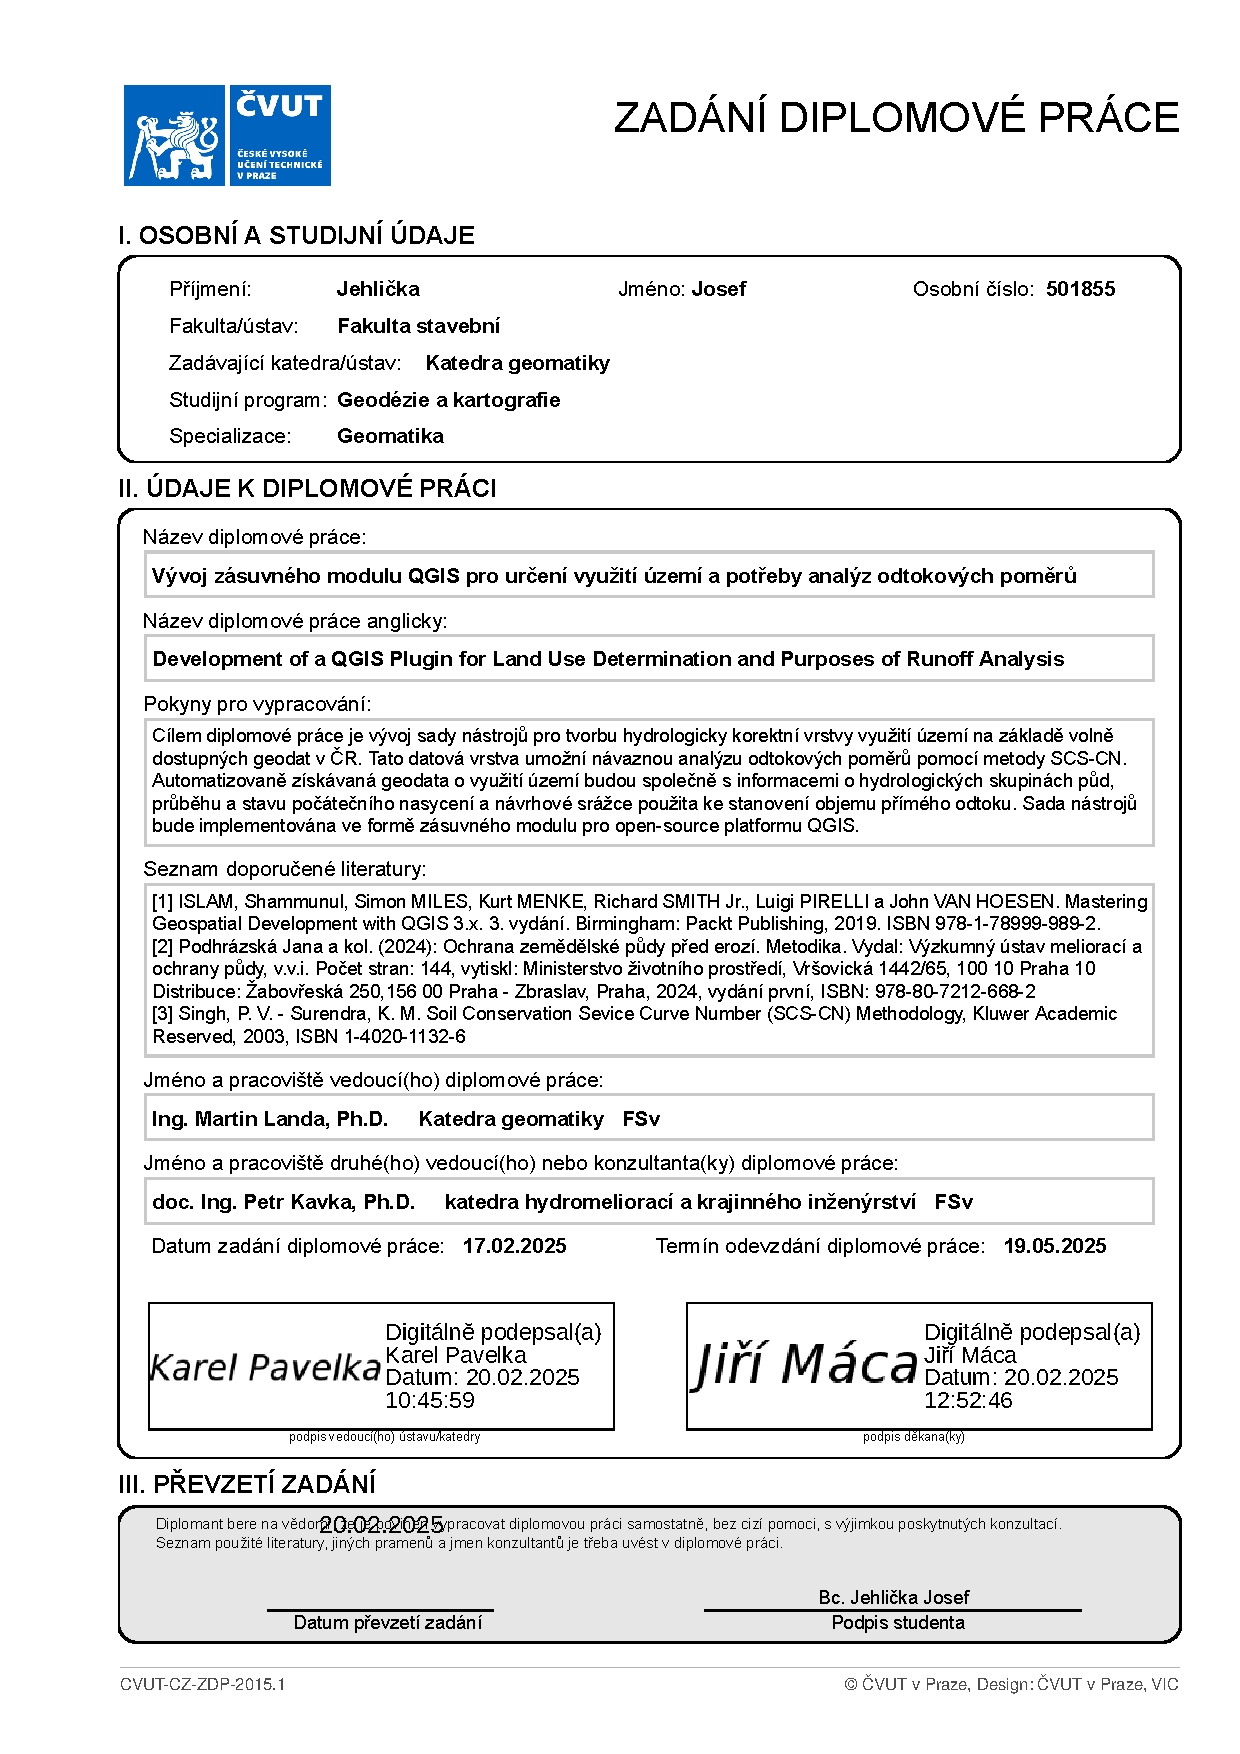
\includepdf[pages={1}]{zadani_cele.pdf} % NAHRAĎTE správným souborem! <<<<<<<<<<<<<<<<<<<<<<<<<





%
%% --- varianta B: zadání naskenované jako jednotlivé stránky:
%\includepdf[pages={1}]{zadani1.pdf} % 1. strana zadání v PDF
%\includepdf[pages={1}]{zadani2.pdf} % 2. strana zadání v PDF
%
%% --- varianta C: zadání naskenované jako 2 samostatné obrázky:
%% 1. strana zadání
%\begin{center}
%     \includegraphics[width=1\textwidth]{zadani1.jpg}
%\end{center}
%% 2. strana zadání
%\newpage  % SEM NESAHEJTE!
%\thispagestyle{empty} % SEM NESAHEJTE!
%\begin{center}
%     \includegraphics[width=1\textwidth]{zadani2.jpg}
%\end{center}







% příprava:    (na následujících 8 řádků NESAHEJTE!)
\newbox\odstavecbox
\newlength\vyskaodstavce
\newcommand\odstavec[2]{%
    \setbox\odstavecbox=\hbox{%
         \parbox[t]{#1}{#2\vrule width 0pt depth 4pt}}%
    \global\vyskaodstavce=\dp\odstavecbox
    \box\odstavecbox}
\newcommand{\delka}{120mm} % šířka textů ve 2. sloupci tabulky

% použití přípravy:    % dovnitř "tabular" vůbec NESAHEJTE!

\section*{ABSTRAKT}
\begin{flushleft}
Tato práce popisuje vývoj zásuvného modulu open-source softwaru QGIS, který provádí přípravu dat a následnou analýzu odtoků SCS-CN  na automatizovaně získávaných volně dostupných geo datech v ČR jako jsou ZABAGED, LPIS a data poskytovaná projektem rain.fsv.cvut.cz. Data jsou ohodnocena podle způsobu využití území a v kombinaci s daty hydrologických skupin půd a hodnotou úhrnu návrhové srážky vstupují do následné analýzy.
\end{flushleft}


\section*{KLÍČOVÁ SLOVA}
\begin{flushleft}
QGIS, SCS-CN, využití území, zásuvný modul, Python, odtok, povodí, GIS, ZABAGED, LPIS
\end{flushleft}


\section*{ABSTRACT}
\begin{flushleft}
This master's thesis describes the development of a plugin for the open-source software QGIS, which performs data preparation and subsequent runoff analysis using the SCS-CN method on automatically acquired freely available geodata in the Czech Republic, such as ZABAGED, LPIS  and data provided by the rain.fsv.cvut.cz project. The data are evaluated based on land use and, in combination with data of hydrologic soil groups and the total design rainfall amount, serve as inputs for the subsequent analysis.
\end{flushleft}


\section*{KEY WORDS}
\begin{flushleft}
QGIS, SCS-CN, land use, plugin, Python, runoff, watershed, GIS, ZABAGED, LPIS
\end{flushleft}

















%%%%%%%%%%%% Prohlášení -- SEM NESAHEJTE! Generuje se automaticky z výše nastavených maker \kde{} a \prohlaseni{}. %%%%%%%%%%%%
\newpage % SEM NESAHEJTE!
\thispagestyle{empty}  % SEM NESAHEJTE!

~ % SEM NESAHEJTE!
\vfill % prázdné místo. SEM NESAHEJTE!
\vspace{1em}
\tb{Prohlášení} % SEM NESAHEJTE!

\vspace{1em} % vertikální mezera. SEM NESAHEJTE!
\prohlaseni

\vspace{2em}  % SEM NESAHEJTE!
\hspace{-0.5em}\begin{tabularx}{\textwidth}{X c}  % SEM NESAHEJTE!
V \kde\ dne .................... &........................................ \\	% SEM NESAHEJTE!
	& \autor
\end{tabularx}	% SEM NESAHEJTE!







\newpage % SEM NESAHEJTE!
\thispagestyle{empty}  % SEM NESAHEJTE!

~
\vfill % prázdné místo


% -- následující kus kódu (do "%%%%%%%%%%%% ABSTRAKT") můžete odstranit, pokud nechcete psát poděkování:
\vspace{1em}
\tb{Poděkování}

\vspace{1em} % vertikální mezera
\podekovani
\begin{flushright}
\autor
\end{flushright}  % <------- tady končí stránka s poděkováním





\newpage
\tableofcontents


\newpage
\chapter*{Úvod} \label{uvod}
\addcontentsline{toc}{chapter}{Úvod}
Technologie GIS usnadňuje práci v nejrůznějších odvětvích průmyslu od precizního zemědělství až po působení bezpečnostních složek. Což může být motivací pro ušlechtilé úsilí určité skupiny vývojářů, takovou pomoc poskytnout zdarma jako otevřený software s možností dodatečného přizpůsobení nebo integrace do externích aplikací. 

Tvorbou zásuvného modulu (pluginu) pro GIS s otevřeným zdrojovým kódem QGIS se zabývá i tato práce. Zmíněný zásuvný modul poskytuje možnost usnadnit práci uživatelům působícím v oblasti hydrologie, konkrétně při výpočtu objemu přímého odtoku metodou SCS-CN na území České republiky. Takové modelování může například být využito při vymezování záplavových území nebo návrzích protipovodňových opatření.

Cílem bylo vytvořit nástroj pro získání dat, ohodnocení území dle jeho využití, kombinaci těchto dat s vrstvou hydrologických skupin půd, doplnění hodnot CN z tabulky a z nich získání objemu přímého odtoku. Uživateli je umožněno v každé části procesu editovat jakékoliv vstupní hodnoty, či upravit nebo použít vlastní geo data. Tento zásuvný modul realizovaný pomocí programovacího jazyka Python je doplněn o dokumentaci a softwarové testy. 

Ačkoliv existují nástroje pro modelování odtokových poměrů metodou SCS-CN, v prostředí volně dostupných GIS řešení chybí specializovaný nástroj, který by kombinoval snadnou použitelnost, integraci s českými datovými zdroji a možnost úprav vstupních parametrů.

Samotná práce popisuje metodu odtokových křivek SCS-CN, software QGIS a s ním propojené softwarové nástroje jako jsou WFS, WPS, jazyk YAML, knihovna PyQt a další. Následně se pak zaměřuje na  datové zdroje volně dostupně v České republice, které jsou ZABAGED a LPIS. Obsahuje též popis prací při vývoji zásuvného modulu. Závěrečná část shrnuje dosažené výsledky, zhodnocuje přínos práce a nabízí možnosti dalšího rozšíření.


\chapter{Metodologie}

\section{Metoda SCS-CN} \label{SCSCN}
\hspace{10mm} Metoda odtokových křivek (SCS-CN) se používá pro určení objemu přímého odtoku. Výhody této metody spočívají v její jednoduchosti a schopnosti reagovat na vlastnosti povodí, jako je typ půdy či využití pozemku (land use). Metoda byla vyvinuta v roce 1954 a publikována v roce 1986 organizací USDA Natural Resources Conservation Service (dříve nazývána Soil Conservation Service). \cite{MNYDGwleJOjKLRUp} Vývoj probíhal na empirických datech získaných v USA, nicméně později byla modifikována na různé typy využití pozemku typické i pro jiné podmínky. \cite{Holman2003}\cite{Lian2020}

\hspace{10mm} Tato metoda může být využita i v menších částech jednotlivých povodí, jejichž rozloha by neměla překročit 10 $km^{2}$ a není vhodná pro výpočet odtoku z tání sněhu. V České republice se využívá hlavně pro návrhy protierozních opatření, a to v souladu s ČSN 75 1400. \cite{MNYDGwleJOjKdRUp}

Výstupem metody CN křivek je hodnota efektivní srážkové výšky dle vzorce (1) \cite{MNYDGwleJOjKdRUp} \cite{MNYDGwleJOjKLRU2} :


\begin{equation}
H_{0} = \frac{\displaystyle (H_{S} - I_{a})^{2}}{\displaystyle H_{S} - I_{a} + A}
\end{equation}

kde:
\begin{tabbing}
    \hspace{10mm} \= $H_{0}$ \hspace{5mm} \= je výška přímého odtoku (mm) \\
    \> $H_{s}$ \> je celkový srážkový úhrn (mm) \\
    \> $I_{a}$ \> je počáteční ztráta (mm) \\
    \> $A$ \> je maximální potenciální retence (mm)
\end{tabbing}

Hodnota počáteční ztráty ($I_{a}$) se určí jako:
\begin{equation}
I_{a} = \lambda A
\end{equation}

\hspace{10mm} Kde $\lambda$ je poměrový koeficient, který se v základu volí $0.2$. Tato hodnota byla empiricky odvozena na povodích na území USA. \cite{Lian2020}\cite{MNYDGwleJOjKLRU2} Takto zvolená hodnota se stala jedním důvodem pro kritiku této metody. \cite{MNYDGwleJOjKLRUp} \cite{MNYDGwleJOjKLRU3} \\

\hspace{10mm} Maximální potenciální retence ($A$) je dále určena na základě CN (curvature number) křivek ze vztahu \cite{MNYDGwleJOjKdRUp} : 
\begin{equation}
A = 25,4 (\frac{1000}{CN}-10)
\end{equation}
\hspace{10mm} Hodnota CN se pohybuje mezi 0 (prakticky 30) až 100. Čím vyšší je hodnota CN, tím větší je pravděpodobnost, že dojde k povrchovému odtoku. Pokud se CN rovná nule, potom představuje teoretickou horní
hranici potenciální retence, což by znamenalo, že takové povodí je nekonečně propustné. \cite{MNYDGwleJOjKLRU3}

\begin{figure}[ht] \label{obr1}
\centering
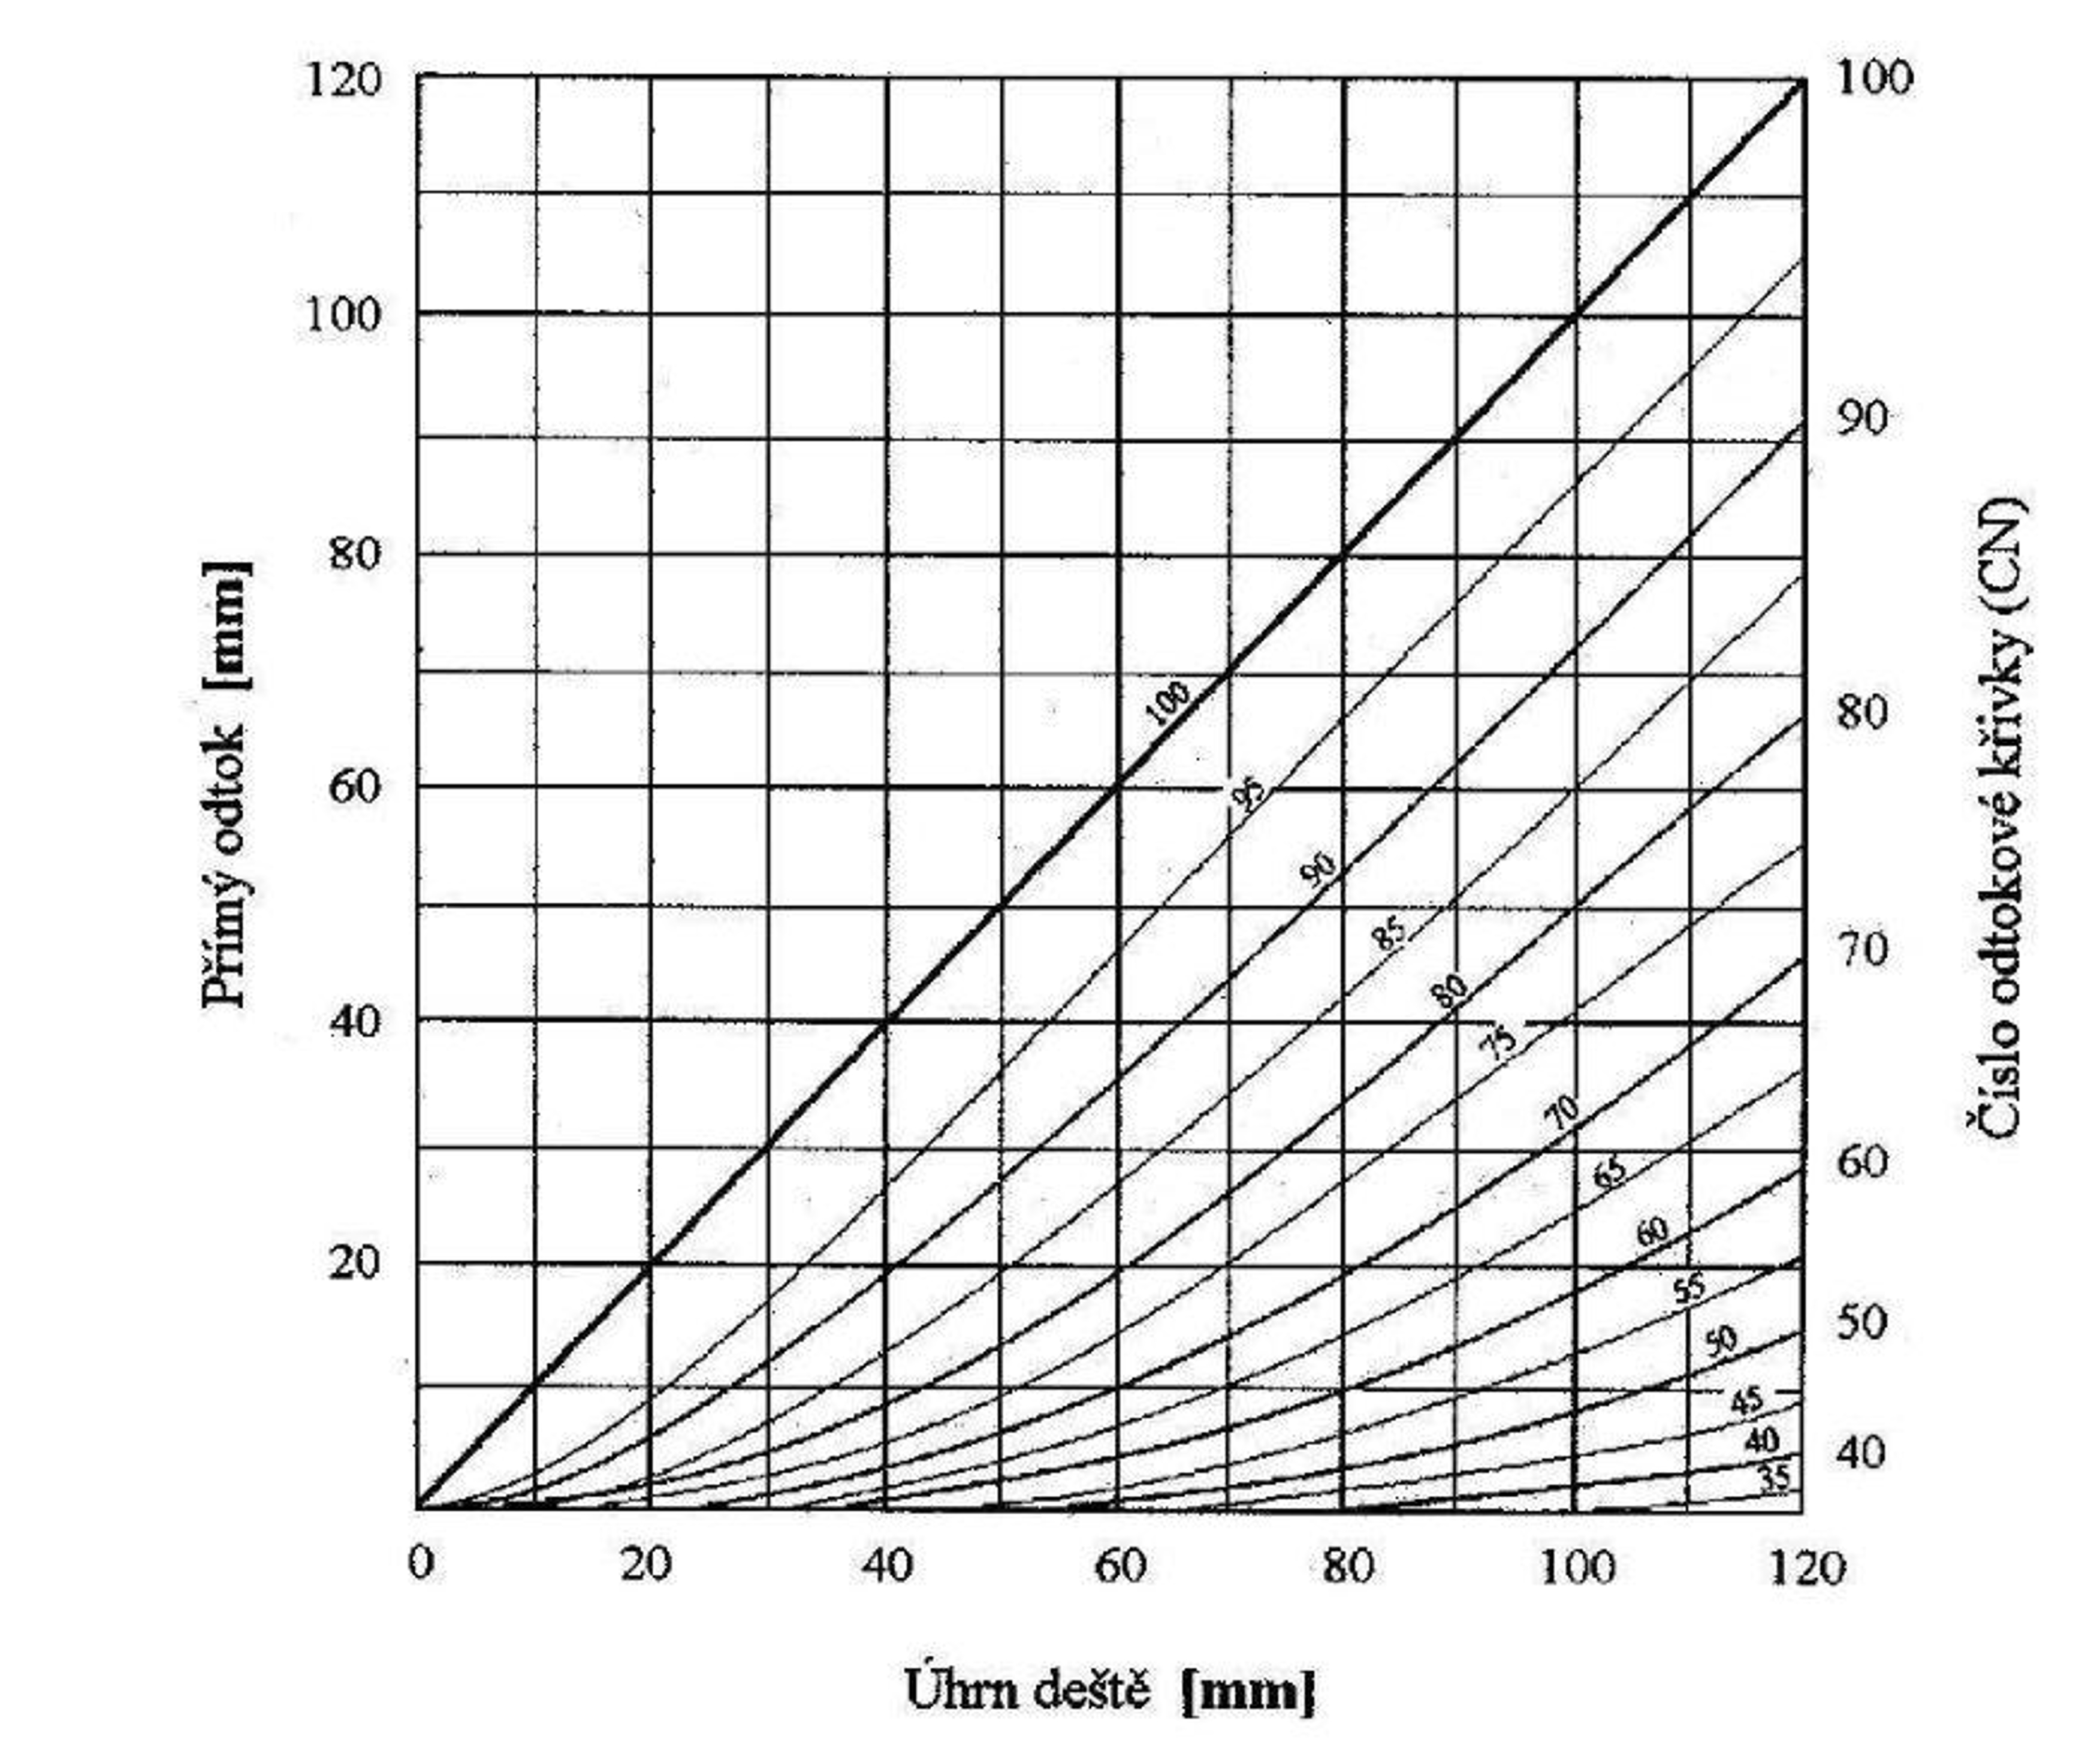
\includegraphics[height=11cm]{pictures/CNcurves.jpg}
\caption{ Závislost výšky přímého odtoku ($H_{o}$) na úhrnu deště($H_{S}$) a číslech odtokových křivek (CN) \textit{(zdroj: Ochrana zemědělské půdy před erozí, Janeček, 2012)}}
\label{fig:example}
\end{figure}

 \hspace{10mm} Tato čísla jsou tabelována pro dvojici jevů. Těmi jsou hydrologické skupiny půd (HSP) a způsob využití území (land use).[4][5][6][7]. V České republice existuje několik tabulek CN hodnot odvozených z originálních USDA hodnot, a to hodnoty dle metodiky Ochrana zemědělské půdy před erozí (rain.fsv.cvut.cz), která je nejnovější platnou metodikou\cite{MNYDGwleJOjKdRUp}. Dříve byly též odvozeny hodnoty CN křivek doporučené v softwaru HydroCad nebo hodnoty CN křivek z projektu QD1368 \cite{Kulasova2004}.

 \hspace{10mm} CN hodnoty jsou také stanoveny pro více počátečních podmínek nasycenosti, a to CN1 pro suché podmínky, CN2 (také pouze CN) pro průměrné podmínky a CN3 pro podmínky vlhké. \cite{dile2016} Nicméně suché podmínky (CN1) na území České republiky prakticky nenastávají \cite{MNYDGwleJOjKdRUp}. Hodnoty CN1 a CN3 lze získat z hodnoty CN2 následovně \cite{Batvari2021}:
 
\begin{equation}
\text{CN}_{1} = \frac{4.2 \, \text{CN}_{2}}{10 - 0.058 \, \text{CN}_{2}}, \quad
\text{CN}_{3} = \frac{23 \, \text{CN}_{2}}{10 + 0.13 \, \text{CN}_{2}}
\end{equation}


\hspace{10mm} Hydrologické skupiny půd (HSP) existují čtyři: A,B,C a D. Do těchto skupin se řadí půda dle minimálních rychlostí infiltrace vody do půdy bez pokryvu a po dlouhodobém nasycení.\cite{MNYDGwleJOjKdRUp}\cite{MNYDGwleJOjKLRU2}
\begin{table}[htbp]
  \centering
  \caption{Tabulka rozdělení do hydrologických skupin půd (HSP) \cite{MNYDGwleJOjKLRU2}} 
  \label{tab:HSP}
  \begin{tabular}{|c|p{6cm}|p{2.5cm}|p{2.5cm}|}
    \hline
    Skupina & Charakteristika hydrologických vlastností [m] & 
    Rychlost infiltrace [mm.min\textsuperscript{-1}] & Rychlost infiltrace [mm.den\textsuperscript{-1}] \\
    \hhline{=|=|=|=|}
    A & Půdy s vysokou rychlostí infiltrace i při úplném nasycení, zahrnující převážně hluboké, dobře až nadměrně odvodněné písky nebo štěrky. & > 0,20 & > 288 \\
    \hline
    B & Půdy se střední rychlostí infiltrace i při úplném nasycení, zahrnující převážně půdy středně hluboké až hluboké, středně až dobře odvodněné, hlinitopísčité až jílovitohlinité. & 0,10–0,20 & 144–288 \\
    \hline
    C & Půdy s nízkou rychlostí infiltrace i při úplném nasycení, zahrnující převážně půdy s málo propustnou vrstvou v půdním profilu a půdy jílovitohlinité až jílovité. & 0,05–0,10 & 72–144 \\
    \hline
    D & Půdy s velmi nízkou rychlostí infiltrace i při úplném nasycení, zahrnující především jíly s vysokou bobtnavostí, půdy s trvale vysokou hladinou podzemní vody, půdy s vrstvou jílu na povrchu nebo těsně pod ním a mělké půdy nad téměř nepropustným podložím. & < 0,05 & < 72 \\
    \hline
  \end{tabular}
  
\end{table}

% Různé zdroje půd (HSP) - velký rozdíl výsledků, je tam graf https://www.vodnihospodarstvi.cz/ArchivPDF/vh2022/vh_09-2022.pdf
\newpage
\section{QGIS} \label{qgis}
\hspace{10mm} QGIS (dříve známý jako Quantum GIS) je jeden z geografických informačních systémů (GIS), tj.  informační systém zabývající se informacemi, které se týkají jevů přidružených k místu vztaženému k Zemi. \cite{dONaeOjXanl1W2md}

\begin{figure}[ht] \label{obr2}
\centering

\includegraphics[height=2cm]{pictures/qgis-logo.png}
\caption{Logo softwaru QGIS}
\label{fig:QGIS}
\end{figure}

\hspace{10mm} Tento software je podporován v prostředí Windows, Mac OS, Linux i Unix. Na rozdíl od komerčních alternativ, jako je například ArcGIS, je QGIS zcela zdarma k použití a řadí se mezi takzvaný otevřený software, který je spravován neziskovou organizací The Open Source Geospatial Foundation (OSGeo).

\begin{figure}[ht] \label{obr3}
\centering

\includegraphics[height=2cm]{pictures/Osgeo.png}
\caption{ Logo organizace OSGeo}
\label{fig:OSGEO}
\end{figure}

\hspace{10mm} OSGeo stojí i za řadou dalších projektů na poli otevřeného softwaru, jako jsou například:
\begin{itemize}
\item GRASS GIS 
\item gvSIG - GIS software
\item PROJ - knihovna pro transformaci souřadnic a kartografických projekcí
\item GDAL/OGR - knihovna pro čtení a zápis GIS formátů
\item PostGIS - SQL pro práci s geoprostorovými daty
\item GeoServer - serverová platforma umožňující publikaci prostorových dat 
\item OpenLayers - JavaScript knihovna pro tvorbu webových mapových aplikací
\end{itemize}


\hspace{10mm} QGIS funguje pod licencí GNU GPL a je postaven na knihovně Qt jazyka C++. QGIS vznikal iniciativou Garyho Shermana, který ji započal v roce 2002 jako prohlížecí software geoprostorových dat pro operační systém Linux. Jeho první verze vyšla až v roce 2009. \cite{Matejova2019}

 \subsection{Zásuvné moduly} \label{moduly}

\hspace{10mm} QGIS je pravidelně jeho vývojáři rozšiřován o nejrůznější funkce, často přejímané z dalších otevřených softwarů jako je například GRASS GIS, GDAL nebo SAGA GIS.\cite{Baghdadi2018}

\hspace{10mm} Nespornou výhodou je i fakt, že jakákoliv nezávislá organizace či jednotlivec může vyvinout vlastní rozšíření tohoto softwaru pomocí zásuvných modulů (tzv. pluginů) využívajících QGIS Python API (PyQGIS). Pokud takto vytvořený modul splní požadavky OSGeo, může být vydán pod její záštitou. Jinak může být distribuován neoficiálně například v komprimovaném adresáři.

\hspace{10mm} Vytvoření takového pluginu zjednodušuje plugin již existující, a to Plugin Builder. Ten je vyvinut společností GeoApt LLC, jejímž vlastníkem je již zmíněný Gary Sherman zakladatel samotného softwaru QGIS. Tento nástroj vytvoří šablonu potřebných souborů pro potřebu vytvoření zásuvného modulu. \cite{QPwvEntkWdxPk0Lz}

\hspace{10mm} Mezi další významné pluginy patří například: OpenLayers Plugin pro zobrazení vrstev Google Maps nebo OpenStreetMap, QuickMapServices pro načítání různých mapových služeb a datových setů, Semi-Automatic Classification Plugin pro řízenou klasifikaci družicových snímků nebo qgis2web pro exportování vrstev do formátu webových stránek. \cite{QPwvEntkWdxPk0Lz}

\hspace{10mm} V prostředí QGIS již existuje zásuvný modul pro analýzu SCS-CN zvaný \textit{Curve Number Generator}, který vytvořil Abdul Raheem Siddiqui. Ten umožňuje volit vstupní datové sady pro Spojené státy americké, globální, či si uživatel může zvolit vlastní rastrová data. Americká datová sada využívá National Land Cover Database, což je rastrová vrstva využití území s rozlišením pixelu 30m a půdní data Soil Survey Geographic Database v měřítku 1:12 000. I dataset pro globální výpočet má na vstupu pouze rastrové vrstvy ESA Land Cover 2021 a ORNL Hydrologic Soil Group dataset. Tento zásuvný modul neobsahuje dokumentaci a neumožňuje navázat výpočtem objemu přímého odtoku. \cite{siddiqui2020}


\section{Datové zdroje} \label{data}
\hspace{10mm} Vstupem pro metodu SCS-CN je kombinace informací o využití území a hydrologických skupinách půd v daném území. Vrstva využití území je v zásuvném modulu získána kombinací vrstev ZABAGED a LPIS. Pro výpočet objemu přímého odtoku je nutno využít i dat srážkových.

\newpage
\subsection{ZABAGED\texorpdfstring{\textsuperscript{\textregistered}}{ (R)}} \label{zabaged}

\hspace{10mm} Základní báze geografických dat České republiky (ZABAGED\texorpdfstring{\textsuperscript{\textregistered}}{ (R)}) je vektorová geografická datová sada ve správě Zeměměřického úřadu ve veřejném zájmu. Skládá se z 140 různých polohopisných geografických objektů, které spadají do následujících kategorií \cite{nEFEg7XpI9hVQCiO} :
\begin{itemize}
\item 1. Sídla, hospodářské a kulturní objekty
\item 2. Komunikace
\item 3. Rozvodné sítě a produktovody
\item 4. Vodstvo 
\item 5. Územní jednotky včetně chráněných území
\item 6. Vegetace a povrch
\item 7. Terénní reliéf
\item 8. Geodetické body
\end{itemize}
\hspace{10mm} Kromě polohopisných dat obsahuje ZABAGED\texorpdfstring{\textsuperscript{\textregistered}}{ (R)} i data výškopisná (vrstevnice, DMR 4G, DMR 5G, DMP 1G) a data spadající pod rámec INSPIRE (Vodstvo, Dopravní sítě, Nadmořská výška GRID, Nadmořská výška TIN). \cite{nEFEg7XpI9hVQCiO} 


\hspace{10mm} Polohopisné objekty jsou distribuovány v různých geometrických zobrazeních:
\begin{itemize}
\item bod
\item centroid plochy
\item linie
\item linie - osa objektu
\item obvodová linie
\item plocha
\end{itemize}

\hspace{10mm} Každý objekt obsahuje atribut o jeho střední polohové chybě vyjádřené v metrech. Původním zdrojem těchto polohových dat je Základní mapa České republiky 1:10 000 (ZM 10). Ta byla několikrát aktualizována pomocí aktuálního Ortofota ČR. Dále se v menší míře využívají data z přímého geodetického měření, data z leteckého laserového
skenování či data od externích subjektů. \cite{nEFEg7XpI9hVQCiO} 


\subsection{LPIS} \label{lpis}
\hspace{10mm} LPIS (Land Parcel Identification System) je geografický informační systém sloužící hlavně k evidenci zemědělské půdy, za něž je odpovědné Ministerstvo zemědělství. Jeho obsahem jsou zemědělské parcely zobrazující vlastnické vztahy. Ty jsou výchozí pro udělování dotací pro zemědělskou půdu.\cite{Devaty2018}

\hspace{10mm} Základní datovou jednotkou je díl půdního bloku (DPB), které jsou zcelovány do souvislých obhospodařovaných ploch tzv. půdních bloků (PB). \cite{Devaty2018}

\hspace{10mm} LPIS je veden ve všech státech Evropské unie, ale v různých státech se pozemky uchovávají v jiných druzích parcel (katastrální parcely, zemědělské parcely, zemědělské půdní bloky nebo fyzické bloky). \cite{KocurBera2019}

Takové plochy obsahují údaje o druhu zemědělské kultury, a to \cite{sSYEwLE0rNKoWGYk}:
\begin{itemize}
    \item orná půda, kterou je
    \begin{itemize}
        \item standardní orná půda,
        \item travní porost a
        \item úhor,
    \end{itemize}
    \item trvalý travní porost,
    \item trvalá kultura, kterou je
    \begin{itemize}
        \item vinice,
        \item chmelnice,
        \item ovocný sad,
        \item školka,
        \item rychle rostoucí dřeviny pěstované ve výmladkových plantážích,
        \item plocha s víceletými produkčními plodinami,
        \item plocha s lanýži a
        \item jiná trvalá kultura, 
    \end{itemize}
    \item ostatní kultura, kterou je
    \begin{itemize}
        \item zalesněná půda,
        \item rybník,
        \item plocha s kontejnery,
        \item mimoprodukční plocha a
        \item jiná kultura.
    \end{itemize}
\end{itemize}

\hspace{10mm} Databáze také obsahuje ekologicky významné prvky a další objekty. \cite{sSYEwLE0rNKoWGYk}
Přístup k těmto datům je zprostředkován webovými službami (iLPIS a pLPIS)  a WMS či WFS službou. \cite{Devaty2018}

\subsection{Hydrologické skupiny půd (HSP)} \label{hsp}
\hspace{10mm}Význam hydrologických skupin půd (Hydrologic Soil Groups) a jejich dělení je popsáno v první kapitole. 
% Různé zdroje půd (HSP) - velký rozdíl výsledků, je tam graf https://www.vodnihospodarstvi.cz/ArchivPDF/vh2022/vh_09-2022.pdf

Zdroje hydrologických skupin půd v České republice existují celkem čtyři \cite{Strouhal2022}:
\begin{itemize}
\item CN (s metodikou výpočtu) dle ČHMÚ (2004)
\item HSP dle projektu „Strategie ochrany před negativními dopady povodní a erozními jevy přírodě blízkými opatřeními v České republice“ (2015)
\item HSP dle VÚMOP (2018) 
\item HSP dle půdní zrnitosti dle projektu „Fyzikální a hydropedologické vlastnosti půd ČR" (2021)
\end{itemize}
\hspace{10mm} Volba zdroje půdních dat může ovlivnit výsledky analýz, nicméně neexistuje způsob, jak určit spolehlivost těchto rozdílných zdrojů dat, přestože se poměrně liší.\cite{Strouhal2022} Proto je doporučeno volit vždy data s méně přívětivými podmínkami v daném území. \cite{MNYDGwleJOjKdRUp} To je vizualizováno níže.

\begin{figure}[H] \label{obr4}
\centering
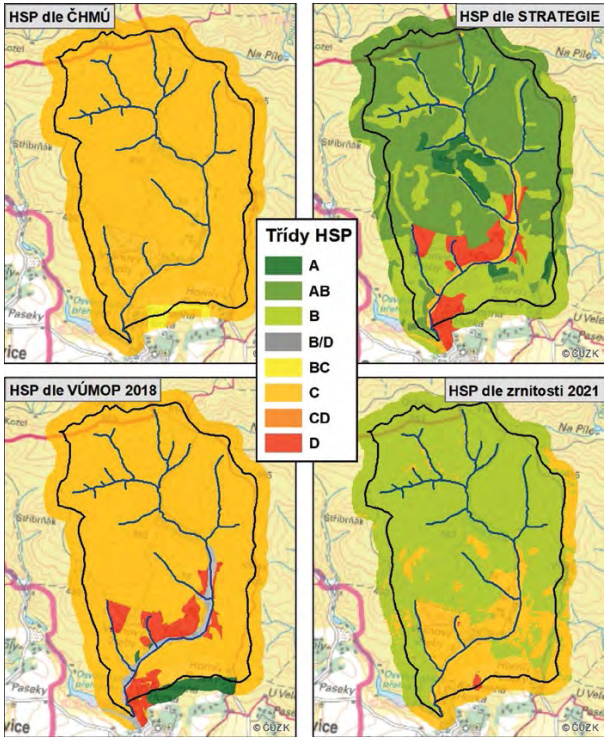
\includegraphics[height=12cm]{pictures/HSPmapa.png}
\caption{Plošné rozdělení jednotlivých HSP na povodí Hruškovice podle různých podkladů \cite{Strouhal2022}}
\label{fig:hsp}
\end{figure}

\newpage
\subsection{Srážková data} \label{rain}
\hspace{10mm} Dle metodik \textit{Krátkodobé srážky pro hydrologické modelování a navrhování drobných vodohospodářských staveb v krajině} \cite{MNYDGwleJOjKLRU2} a \textit{Ochrana zemědělské půdy před erozí} \cite{MNYDGwleJOjKdRUp} je žádoucí navrhovat protipovodňová opatření pro velikost návrhového šestihodinového úhrnu srážek v šesti alternativách jejich průběhu, vyjádřených sestavou šesti syntetických hyetogramů. 

\hspace{10mm} Pokud je tedy návrhová srážka odvozena pro nějakou dobu opakování, je možné z ní vypočtený objem přímého odtoku v kombinaci se šesti tvary  hyetogramů a pravděpodobností abnormálního předchozího nasycení vážit.

\hspace{10mm} To znamená, že výsledný objem je vypočten z hodnot \textit{CN2} i \textit{CN3} (viz Kapitola 1.1), s uvážením pravděpodobnosti obou scénářů počátečního nasycení.

\hspace{10mm} Úhrny návrhových srážek, tvary hyetogramů a pravděpodobnosti abnormálního předchozího nasycení pro různé doby opakování se šestihodinovými úhrny jsou poskytovány portálem \textit{rain.fsv.cvut.cz}.

\newpage
\newpage

\section{Použité technologie} \label{tehcnologie}

\subsection{Web Feature Service (WFS)} \label{wfs}
\hspace{10mm} Web Feature Service je internetová služba pro šíření geografických informací, která nahradila šíření celých datových souborů například pomocí File Transfer Protocol (FTP). Služba je standardizována organizací Open Geospatial Consortium (OGC) v dokumentu  ISO 19119. \cite{Vretanos2014} WFS je implementována v jazyce XML a data jsou reprezentována primárně v jazyce GML. \cite{Zhang2005}

\hspace{10mm} Na rozdíl od Web Map Service (WMS), která připojuje vrstvy jako needitovatelné rastrové podkladové vrstvy, WFS slouží ke sdílení vektorových dat s možností následné editace. Uživatel zašle požadavek ve formátu XML na WFS server, který vrátí odpověď opět v XML. \cite{Zhang2005}

\begin{figure}[ht] \label{obr5}
\centering
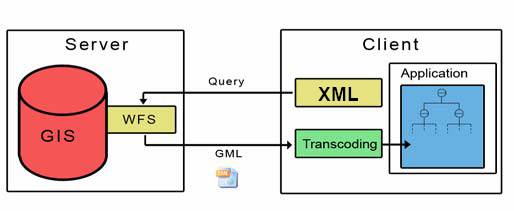
\includegraphics[height=6cm]{pictures/XML.png}
\caption{Schéma služby WFS \cite{Schall2009}}
\label{fig:xml}
\end{figure}

\hspace{10mm} Pro komunikaci se serverem poskytující WFS službu může uživatel využít následujících jedenáct operací:

\begin{table}[htbp]
  \centering
  \caption{Tabulka WFS operací} 
  \label{tab:WFS}
  \begin{tabular}{|c|c|p{7cm}|}
    \hline
    \textbf{Operace} & \textbf{Volitelný} & \textbf{Popis} \\
    \hhline{=|=|=}
    GetCapabilities & NE & Načte metadata o službě, včetně podporovaných operací a parametrů, a seznam dostupných typů prvků. \\
    \hline
    DescribeFeatureType & NE & Vrací popis struktury typů prvků a jejich vlastností, které WFS poskytuje nebo přijímá. \\
    \hline
    GetFeature & NE & Vrací výběr instancí prvků z datového úložiště publikovaného prostřednictvím WFS. \\
    \hline
    ListStoredQueries & NE & Vrací seznam dotazů, které byly uloženy v instanci WFS. \\
    \hline
    DescribeStoredQueries & NE & Vrací popis dotazů, které byly uloženy v instanci WFS. \\
    \hline
    GetPropertyValue & ANO & Načítá hodnotu vlastnosti prvku nebo část hodnoty složité vlastnosti pro sadu prvků. \\
    \hline
    GetFeatureWithLock & ANO & Podobné jako GetFeature, ale s možností uzamknout prvek pro následné úpravy. \\
    \hline
    LockFeature & ANO & Uzamkne sadu instancí prvků tak, aby je jiné operace nemohly měnit, dokud je zámek aktivní. \\
    \hline
    Transaction & ANO & Umožňuje modifikaci nebo odstranění instancí prvků a jejich vlastností. \\
    \hline
    CreateStoredQuery & ANO & Vytvoří a uloží dotaz, který může klient snadno vyvolat později. \\
    \hline
    DropStoredQuery & ANO & Odstraní dříve uložený dotaz ze serveru. \\
    \hline
  \end{tabular}
\end{table}

\subsection{Web Processing Service (WPS)} \label{wps}
\hspace{10mm}Web Processing Service (WPS) je služba umožňující nad poskytnutými daty provést jakoukoliv GIS operaci, a to od bufferu až po generování analytických modelů. Komunikace probíhá stejně jako u WFS pomocí XML. K tomu může být využita knihovna OWSLib.

\hspace{10mm}Tato služba standardizovaná OGC může komunikovat s jednou a více WFS službami, pro získání dodatečných geo dat. \cite{Stollberg2007} WPS může také poskytované procesy monitorovat a případně je ukončit. \cite{5Xjhvf3W3tsG6nhX} 

\begin{figure}[ht] \label{obr6}
\centering
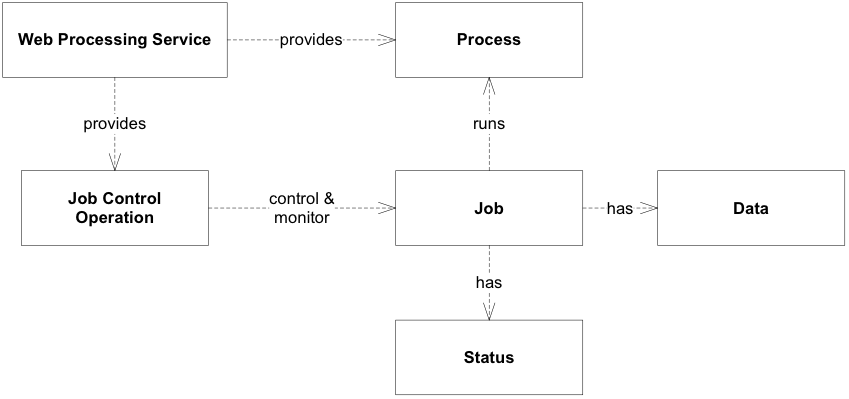
\includegraphics[height=7cm]{pictures/WPS.png}
\caption{Konceptuální model WPS \cite{5Xjhvf3W3tsG6nhX}}
\label{fig:wps}
\end{figure}


\subsection{YAML formát} \label{yaml}



\hspace{10mm}YAML (YAML Ain’t Markup Language) je jazyk pro serializaci dat. Je tvořen tak, aby byl čitelný a pohodlný pro užívání s řadou novodobých programovacích jazyků. Informace uchovává v Unicode charakterů strukturovaných v hodnotových párech a  odrážkových seznamech.  \cite{hsOq0virmVAO85Ud}
\begin{figure}[ht] \label{obr7}
\centering

\includegraphics[height=3cm]{pictures/yaml.png}
\caption{Logo projektu YAML  (zdroj: Wikimedia Commons)}
\label{fig:yaml}
\end{figure}

\hspace{10mm}YAML se od XML liší tím, že je vytvořen hlavně pro ukládání dat, zatímco XML slouží k uložení uspořádaných dokumentů. YAML je lépe čitelný díky odsazení a chybějícím znaménkům zatímco XML používá složitější syntaxi. \cite{hsOq0virmVAO85Ud}

\hspace{10mm}YAML je také jednoduší pro editaci člověkem než JSON, který je vhodnější pro zpracování strojem. YAML může mít složitější datové struktury a využívá komentáře, ale JSON má jednodušší pravidla. \cite{hsOq0virmVAO85Ud}


\subsection{Python knihovna PyQt} \label{pyqt}
\hspace{10mm}PyQt je sada Python příkazů pro multiplatformní aplikační vývojovou platformu, která kombinuje všechny výhody Qt a Pythonu.  \cite{Summerfield2007}

\begin{figure}[ht] \label{obr8}
\centering

\includegraphics[height=3cm]{pictures/Python_and_Qt.png}
\caption{Kombinace log Python a Qt  (zdroj: Wikimedia Commons)}
\label{fig:qt}
\end{figure}

\hspace{10mm}Qt je aplikační rámec pro tvorbu uživatelských prostředí podporující řadu hardwaru a operačních systémů. Tvorbu uživatelského prostředí zprostředkovávají softwary jako jsou QtCreator nebo QtDesigner, jehož specializovaná verze je součástí instalace QGIS.

\hspace{10mm}PyQt umožňuje propojit Python kód s množstvím prvků uživatelského prostředí, jako jsou tlačítka, popisky, přepínače, zaškrtávací políčka, rozbalovací seznamy nebo okna pro vstup textu.

\subsection{Python knihovna pytest} \label{pytest}
\hspace{10mm}Robustní knihovna pytest se používá pro všechny druhy testování softwaru. Od konkurenční knihovny unittest na tuto přešla spousta projektů, jako jsou třeba Mozilla nebo Dropbox. \cite{Okken2017}

\begin{figure}[ht] \label{obr9}
\centering

\includegraphics[height=4cm]{pictures/Pytest_logo.png}
\caption{Logo knihovny pytest [24]}
\label{fig:pytest}
\end{figure}

\hspace{10mm}Výhody knihovny jsou například nezávislost na verzi Pythonu, snadná čitelnost a implementace nebo otevřenost zdrojového kódu pod licencí MIT. Díky tomu byla pro knihovnu vyvinuta řada zásuvných modulů pro specifičtější použití. \cite{Okken2017}

\hspace{10mm}Testy je možné spouštět přímo v příkazové řádce, přičemž je uživatel informován o prostředí, ve kterém je test spuštěn, době jeho trvání a počtu procházejících a selhávajících úkonů.   

\newpage
\subsection{GitHub} \label{github}
Tato vývojářská platforma umožňuje vzdálené uložení a editaci kódu. Na její pozadí stojí Git, což je systém pro správu verzí. Ten byl původně vytvořen Linusem Torvaldsem, aby usnadnil vývoj jádra operačního systému Linux. \cite{Guthals2023}

\begin{figure}[ht] \label{obr10}
\centering

\includegraphics[height=4cm]{pictures/git.png}
\caption{Logo platformy GitHub (vlevo) a systému Git (vpravo) \cite{Guthals2023}}
\label{fig:git}
\end{figure}

\hspace{10mm}Na stránkách GitHub je možné po založení účtu vytvořit repozitář pro daný projekt. Při vývoji lze vytvářet nové vývojové větve (branch), které je možné zařadit do větve hlavní. Tímto způsobem může na projektu spolupracovat více lidí najednou a nezávisle. Výhodou je také fakt, že v každé větvi je možné provedené změny vrátit do původního stavu. Tento proces lze zjednodušeně přiblížit na úpravě textového dokumentu více uživateli ve službě Google Docs. \cite{Guthals2023}

\hspace{10mm}Při zapojení (\textit{merge}) vedlejší větve s úpravami do hlavní lze vytvořit žádost o začlenění změn (\textit{pull-request}), kde může více uživatelů diskutovat o provedených změnách. \cite{Guthals2023}

\hspace{10mm}GitHub je možné propojit s velkým množstvím vývojových prostředí nebo je možné využít aplikaci GitHub Desktop pro klonování repozitářů na lokální úložiště. Nicméně stejné funkcionality lze dosáhnout užitím pouze
příkazové řádky. 

\hspace{10mm}Pomocí služby GitHub Actions lze repozitář propojit s nějakou externí funkcionalitou, mezi které patří: vytvoření Python knihovny, vytvoření Dockeru, propojení s externími cloudovými službami, spouštění testů nebo vytvoření webových stránek ze souborů repozitáře. 
\newpage
\subsection{Markdown a MkDocs} \label{markdown}

\begin{figure}[H] \label{obrmd}
\centering

\includegraphics[height=3cm]{pictures/md.png}
\caption{Logo nástroje MkDocs (vlevo) a značkovacího jazyka Markdown (vpravo) \cite{Guthals2023}}
\label{fig:md}
\end{figure}

\hspace{10mm} Značkovací jazyk Markdown je účinný nástroj pro dodání formátovacích prvků do jednoduchých textových dokumentů. Vytvořil ho John Gruber v roce 2004 a je jedním z nejrozšířenějších značkovacích jazyků. \cite{Cone2020}

\hspace{10mm} Markdown nepatří mezi takzvané WYSIWYG (\textit{What You See Is What You Get}) editory, jako je například MS Word nebo LibreOffice Writer. Markdown soubor je potřeba nejprve zkompilovat, aby jeho formátování bylo zřetelné. Zkompilovat ho lze různými nástroji nejen do PDF, ale i HTML formátu. \cite{Cone2020}

\hspace{10mm}V tomto formátu lze tvořit nejrůznější úpravy textu jako nadpisy, tučné písmo, kurzívu, odrážkové seznamy a spoustu dalších. Je umožněno také vkládat obrázky a kombinovat Markdown s HTML. \cite{Cone2020}

\begin{figure}[H]
\begin{pythoncode}[style=mypython, caption={Ukázka Markdown syntaxe},label={kod:md}]
# Nadpis nejvyšší úrovně
Odstavec s **tučným** a *šikmým textem*
1. číslovaný seznam
2. s několika
2. položkami

## Podnadpis <h2>
Zdrojový kód může být `v řádku` nebo jako blok:

  Výpis zdrojového kódu.
> Bloková citace
- nečíslovaný
- seznam
\end{pythoncode}
\end{figure}

\hspace{10mm} MkDocs je nástroj, který z Markdown souborů dokáže generovat statické webové stránky se zaměřením na tvorbu dokumentace různých projektů. Uživatel má možnost si vybrat z řady grafických šablon vyvíjených komunitou.

\hspace{10mm}MkDocs obsahuje i vestavěný server s živým náhledem všech provedených změn. Do prostředí je umožněno také přidávat uživatelské nástavby různých editací textu nad rámec jazyka Markdown.


\chapter{Postup implementace} \label{implementace}
\hspace{10mm}Všechny kroky implementace byly uskutečněny v rámci GitHub repozitáře spadajícího pod organizaci GeoForAll Lab at CTU in Prague.

\section{Návrh pracovního postupu} \label{workflow}
\hspace{10mm}Nejprve bylo nutné zajistit způsob, jakým bude uživatel definovat zájmovou oblast pro průběh analýzy. Vhodně se jevilo, aby bylo možné zvolit oblast buď uvnitř již existujícího polygonu nebo zjednodušeně ve výřezu okna obrazovky.

\hspace{10mm}Geometrické a polohové vlastnosti těchto objektů bylo nutné následně předat službám WPS a WFS, které zajišťují získávání dat od třetích stran. Po získání vektorových dat ze služeb WFS poskytovaných správci datových sad ZABAGED a LPIS se jevilo žádoucí aplikovat buffer na liniové či bodové prvky s předpokladem, že tyto buffery se budou řídit atributovými hodnotami takových vrstev (například třída nebo typ pozemní komunikace). 

\hspace{10mm}Všem polygonovým vrstvám je následně potřeba přiřadit kód využití území. Základní dle názvu vrstvy a detailnější hodnotu dle různých hodnot atributů (příkladem může být třeba vrstva lesa, které byla přidána základní hodnota a přírůstky k této hodnotě dle atributu druhu lesa).

\hspace{10mm}Po těchto úpravách následuje proces oříznutí vrstev, tak aby přesně kopírovaly definiční polygon zájmového území na vstupu a aby prvky po aplikovaném bufferu tento polygon či výřez obrazovky nepřesahovaly.

\hspace{10mm}Dále existuje potřeba tyto vrstvy spojit do jedné dle dané priority. Například tak, aby komunikace vedly nad vodními toky, budovy se nacházely nad zastavěnou plochou a podobně.

\hspace{10mm}Druhou potřebnou vrstvou vstupující do výpočtu je vrstva obsahující hydrologické skupiny půd (HSG). Ta je získávána z WPS služby umístěné na adrese rain.fsv.cvut.cz. Tato služba umožňuje získávat půdní data v rastrové podobě, a proto následuje proces jejich polygonizace. Taková vrstva je také oříznuta dle zájmového území.

\hspace{10mm}Pomocí geometrického sjednocení vstupních prvků jsou obě vrstvy spojeny do jedné se zachovanými atributy o hydrologických skupinách půd a využití území.
Z jejich kombinace se poté dle zvolené tabulky přiřadí hodnoty CN.

\hspace{10mm} Následuje potřeba začlenit možnost vytvořit vrstvu s výškami a objemy přímého odtoku. Zde by mělo být uživateli umožněno vybrat z aktivního projektu vrstvu CN hodnot.

\hspace{10mm} Mezi další vstupy je vhodné definovat hodnotu poměrového koeficientu počáteční ztráty ($\lambda$) a jednu či více hodnot výšek úhrnů.

\hspace{10mm} Výpočet by dále měl umožňovat využít výšek úhrnů poskytovaných WPS službou umístěnou na \textit{rain.fsv.cvut.cz} pro různé doby opakování.  
Z objemů přímých odtoků pro tyto doby opakování a z hodnot CN2 a CN3 se pak dle pravděpodobností tvarů hyetogramů a abnormálního nasycení získá vážený objem přímého odtoku, přičemž všechny tyto hodnoty opět poskytuje WPS služba.

\begin{figure}[H] \label{obr11}
\centering
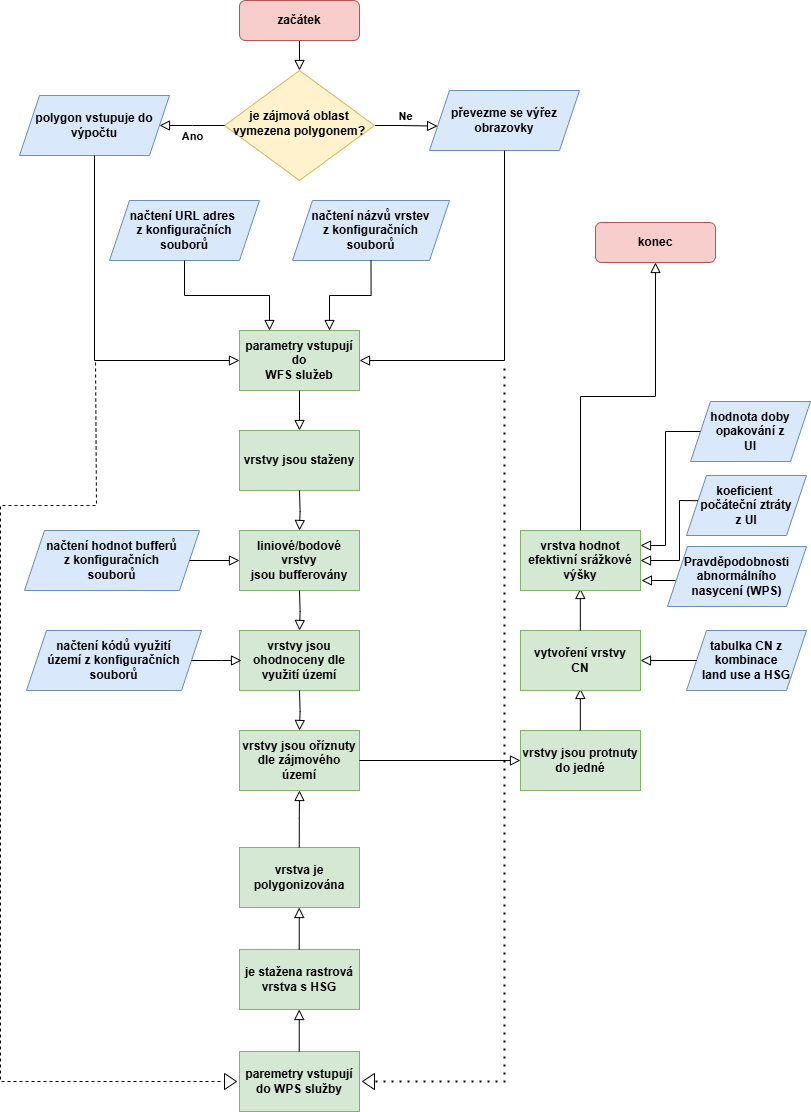
\includegraphics[height=21cm]{pictures/diagram.png}
\caption{Vývojový diagram pracovního postupu}
\label{fig:diagram}
\end{figure}

\section{Tvorba grafického uživatelského rozhraní} \label{gui}

\hspace{10mm} Pro generaci základních souborů pluginu, nutné pro otevření okna Qt objektu \textit{QDockWidget} a další užitečné integrace se softwarem QGIS, byl využit zásuvný modul \textit{Plugin Builder}. 

\hspace{10mm} Zde bylo možné nastavit název modulu, jenž byl zvolen jako \textit{Czech Land Use and CN Analyzer}, jeho krátký popis, číslo jeho verze, jméno autora, kontaktní email nebo odkazy na domovskou stránku a repozitář. Tyto popisující prvky se následně ukáží u pluginu v QGIS správci zásuvných modulů.

\hspace{10mm} Pluginu byla též vytvořena ikona a pomocí nástroje \textit{pb\_tool} byl adresář pluginu překompilován pro její implementaci.

\begin{figure}[H] \label{obr12}
\centering

\includegraphics[height=2cm]{pictures/icon.png}
\caption{Ikona zásuvného modulu}
\label{fig:icon}
\end{figure}

\hspace{10mm} Následně byl upraven panel zásuvného modulu v softwaru Qt Designer, který je možné stáhnout společně s instalací softwaru QGIS. Tato jeho verze obsahuje nástavbu s speciálními objekty specifické pro GIS prostředí. Prvně byl do okna pluginu přidán panel se záložkami.

\hspace{10mm} Záložky byly vytvořeny čtyři: první pro stažení dat, druhá pro výběr a propojení vrstev využití území a hydrologických skupin půd, třetí pro vytvoření vrstvy s hodnotami CN a čtvrtá pro výpočet objemu přímého odtoku.

\hspace{10mm} První záložka umožňuje uživateli vybrat, zda stažení dat proběhne uvnitř výřezu obrazovky nebo uvnitř polygonu. V případě stažení uvnitř polygonu si uživatel může zvolit vrstvu, kterou chce pro definici zájmového území využít. Na toto okno je nastaven filtr, aby zobrazovalo pouze vektorové vrstvy.

\hspace{10mm} Dále si může vybrat, zda chce stáhnout vrstvu využití území, vrstvu hydrologických skupin půd nebo obě.  Proces stahování je možné zahájit tlačítkem, jeho postup se zobrazuje v ukazateli průběhu a je možně jej ukončit tlačítkem (\textit{Abort}) mezi jednotlivými vrácenými vrstvami.  

\hspace{10mm} V druhé záložce jsou dvě rozbalovací okna s filtry pro zobrazení pouze vektorových vrstev, kde je možné vybrat z projektu vrstvy využití území a hydrologických skupin půd. Tlačítkem níže je možné tyto vrstvy propojit do jedné. Obě vrstvy jsou po stažení automaticky přidávány do daných rozbalovacích oken.

\begin{figure}[H] \label{obr12a}
\centering
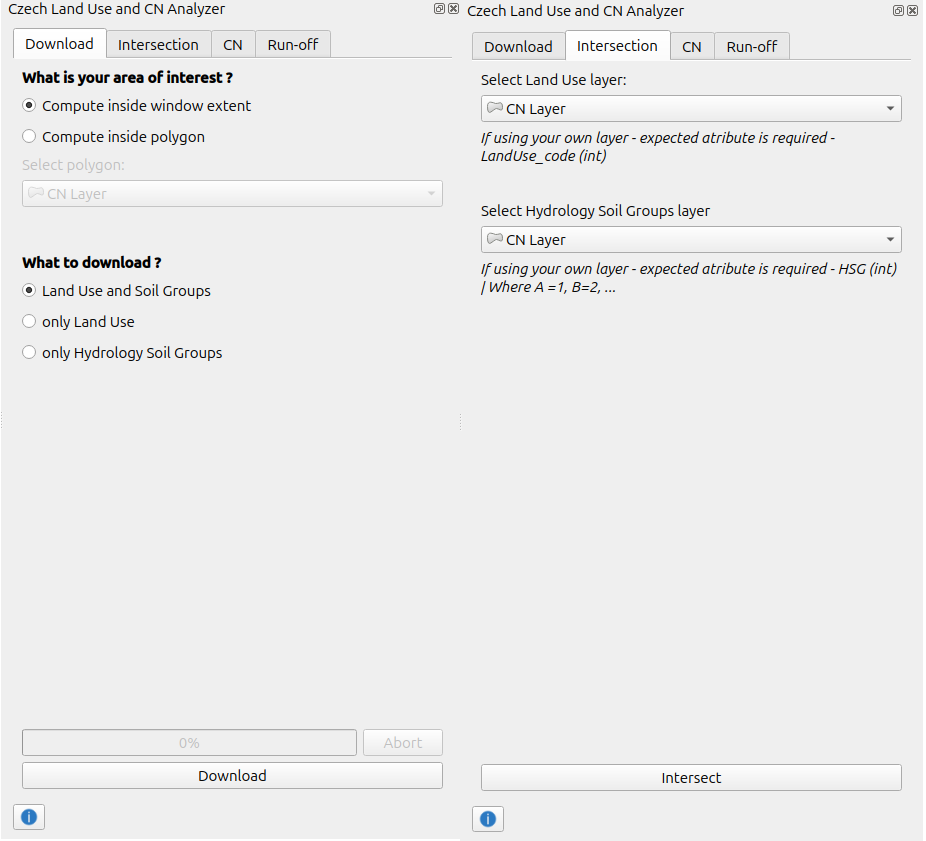
\includegraphics[height=9cm]{pictures/UI1.png}
\caption{Ukázka první (vlevo) a druhé (vpravo) záložky modulu }
\label{fig:UI1}
\end{figure}

\hspace{10mm} Uvnitř třetí záložky je rozbalovací okno pro výběr propojené vrstvy využití území a hydrologických skupin půd, která je do něj automaticky vložena po jejím vytvoření v předchozí záložce. Dále je zde cesta k základní tabulce CN hodnot, která může být změněna dialogem výběru souboru spustitelným bočním tlačítkem.

\hspace{10mm} Čtvrtá záložka opět obsahuje rozbalovací okno pro výběr CN vrstvy. Dále se zde nachází pole pro vstup textu, kde je nutné vložit poměrový koeficient počáteční ztráty ($\lambda$), v němž je nastavena základní hodnota 0,2.

\hspace{10mm} Poté si uživatel může pomocí přepínače vybrat, zda chce pro výpočet použít vlastní návrhovou výšku úhrnu nebo využít návrhové výšky úhrnu pro jednotlivé doby opakování. Vlastní výšku úhrnu může zadat do textového pole a pro výpočet z více výšek úhrnu zároveň může tyto hodnoty oddělit symbolem středníku. Při výpočtu pro různé doby opakování si může uživatel ty, pro které požaduje výsledek, zvolit zaškrtávacími tlačítky.

\hspace{10mm} Pod panelem se záložkami se nachází modré tlačítko, kterým je možné zobrazit dokumentaci ve webovém prohlížeči.

\begin{figure}[H] \label{obr12b}
\centering
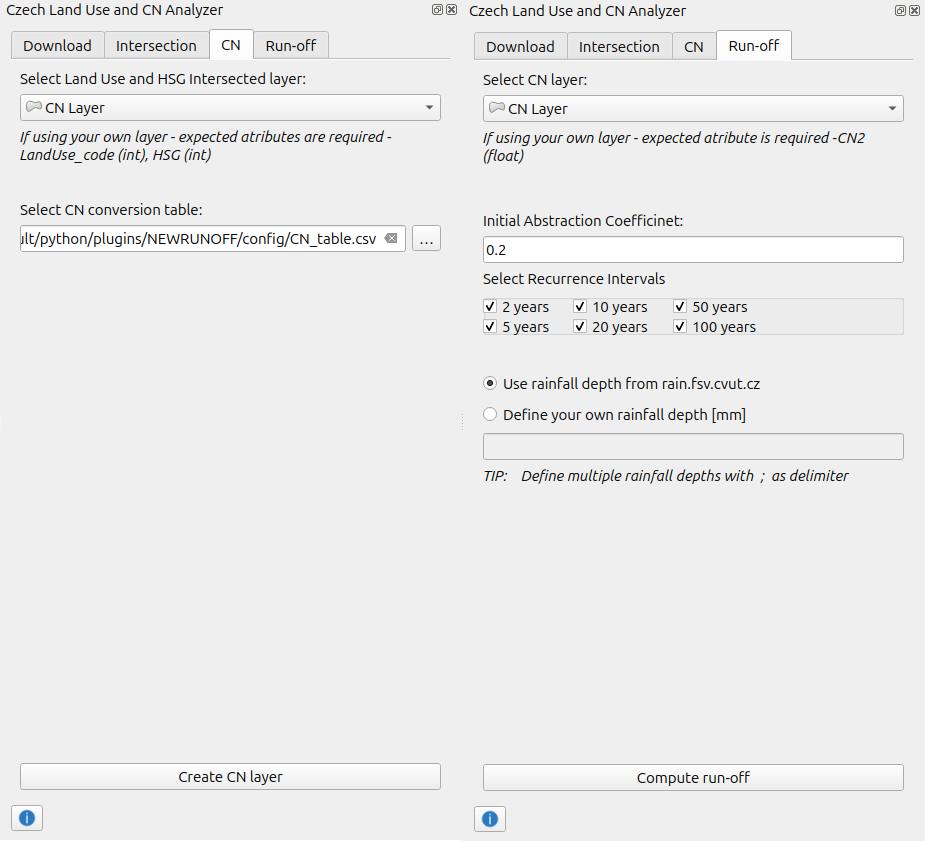
\includegraphics[height=9cm]{pictures/UI2.png}
\caption{Ukázka třetí (vlevo) a čtvrté (vpravo) záložky modulu }
\label{fig:UI2}
\end{figure}


\section{Získávání vrstvy využití území (land use)} \label{landuse}
\hspace{10mm}Nejprve je nutné získat územní rozsah, ve kterém se budou získávat potřebné vrstvy. Podle volby uživatele v grafickém uživatelském rozhraní se použije buď výřez obrazovky, nebo ohraničující obdélník vybraného polygonu. 

\begin{figure}[H]
\begin{pseudocode}[style=mypseudocode, caption={Získání územního rozsahu}, label={kod:extent}]
POKUD uživatel zadal výřez obrazovky
    rozsah @ souřadnice rohů výřezu obrazovky
JINAK POKUD polygon existuje A polygon je validní
    rozsah @ rozsah polygonu
JINAK 
    Uživatel je varován o neplatné vrstvě
    Ukončení procesu stahování
KONEC PODMINKY

VRATIT rozsah

\end{pseudocode}
\end{figure}

\hspace{10mm}Z konfiguračních souborů je poté načten seznam názvů a URL adresy WFS služeb stahovaných vrstev. Všechny tyto parametry jsou přesunuty do jiného vlákna softwaru QGIS, kvůli zachování responsivity samotné aplikace QGIS při procesu stahování. Na pozadí je potom stažena z WFS služby každá vrstva z dříve získaného seznamu vrstev v požadovaném rozsahu. Každou získanou vrstvou se také přiřadí nová hodnota v ukazateli průběhu v uživatelském rozhraní.

\begin{figure}[H]
\begin{pseudocode}[style=mypseudocode, caption={Stažení vrstvy z WFS služby}, label={kod:wfs}]
URI @ kombinace z URL, požadavku GetFeature, název vrszvy, rozsah, EPSG
vektorová vrstva @ Načtení URI do vektorové vrstvy v paměti
vektorová vrstva @ oříznutí vrstvy dle polygonu nebo výřezu obrazovky
POKUD vektorová vrstva je validní
    VRATIT vektorová vrstva
JINAK
    varování uživatele: "Oříznutá vrstva není validní"
    VRATIT 
KONEC PODMINKY
\end{pseudocode}
\end{figure}

\hspace{10mm}Takto získané vrstvy se uchovají v paměti počítače a nyní je potřeba provést kroky, aby jednotlivé vrstvy reprezentovaly využití území. K jednoznačné identifikaci typu využití území se využije kód, který se zároveň bude vyskytovat v tabulce pozdější funkcionality určení hodnoty CN. V první fázi přiřazení se u každé vrstvy vytvoří atribut pro hodnotu kódu využití území a doplní se jeho základní hodnota dle názvu vrstvy. Rozlišné vrstvy mohou mít i totožný kód využití území, jako například silnice a parkoviště, jelikož se v obou případech jedná o antropogenní nepropustné povrchy. Tato hodnota je přiřazena pomocí klíčového slova v názvu vrstvy, ke kterému je v konfiguračním souboru přiřazena hodnota kódu využití území. Díky tomu bude tato funkcionalita zachována i v případě, že správce WFS služby obmění názvy poskytovaných vrstev.

\begin{figure}[H] \label{obr17}
\centering
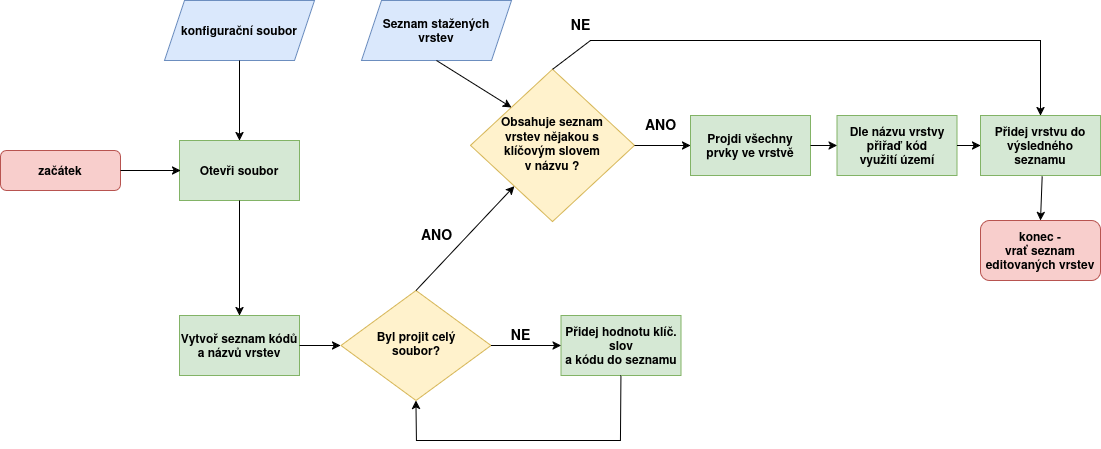
\includegraphics[height=6cm]{pictures/LUcode_diagram.png}
\caption{Vývojový diagram přiřazení kódu využití území dle názvu vrstvy}
\label{fig:LU_diagram}
\end{figure}

\hspace{10mm}Některé stahované vrstvy jsou liniové nebo bodové a právě na ně je aplikován buffer. Pro mnohé je aplikován jen pouze dle názvu vrstvy a pro některé je hodnota bufferu přiřazena dle vybraného řídícího atributu. Pokud řídící atribut obsahuje nečekané hodnoty nebo neobsahuje hodnotu žádnou, je zvolena definovaná implicitní velikost bufferu.

\begin{figure}[H]
\begin{pseudocode}[style=mypseudocode, caption={Přiřazení velikosti bufferu}, label={kod:buffer}]
PRO KAŽDÝ prvek v kolekci prvků vrstvy:
    Získej hodnotu řídícího atributu prvku
 
    POKUD je hodnota řídícího atributu v konfiguračním souboru:
        vyhledej hodnou bufferu
        Přiřaď hodnotu bufferu
        Aplikuj buffer
    JINAK:
        Přiřaď implicitní hodnotu bufferu
        Aplikuj buffer
    
KONEC CYKLU
\end{pseudocode}
\end{figure}

\hspace{10mm}Další implementovanou funkcí pluginu je  zpřesnění kódu využití území dle nějakého atributu vrstvy. Jelikož atribut u vrstvy nemění přiřazený kód z názvu vrstvy, tak se k již přiřazené hodnotě pouze přičte žádané číslo. Jestliže atribut obsahuje neočekávanou hodnotu, zůstane u prvku pouze základní kód.

 \hspace{10mm}Po těchto úpravách je na řadě oříznutí vrstev tak, aby po aplikovaném bufferu nezasahovaly mimo zájmové území. Následně je potřeba všechny vrstvy spojit do jedné podle požadovaného pořadí. 
 
  \hspace{10mm} Toho je docíleno úpravou každé vrstvy v kombinaci s jednou vrstvou o úroveň výše, s tím že vrstva nejvýše není editována. Na každou dvojici vrstev je použit symetrický rozdíl (\textit{symmetrical difference}) a jejich překrytové části jsou odstraněny. Po této úpravě jsou spojeny do jedné a slouží k určení rozlohy prvků o úroveň níže, dokud nevznikne jediná vrstva, kde se žádné prvky nepřekrývají.
  
 Na finální spojenou vrstvu využití území je pak aplikována tabulka symbologie a je přidána do projektu.
 
\section{Získání vrstvy HSP a její propojení s vrstvou využití území} \label{intersection}
 \hspace{10mm}Data hydrologických skupin půd využitých v zásuvném modulu jsou získávány z WPS služby umístěné na doméně \textit{rain.fsv.cvut.cz} . Tato služba má na vstupu polygonovou vrstvu s maximálním rozsahem 20 $km^2$ a názvy požadovaných vrstev. Tato služba totiž nabízí kromě dat hydrologických skupin půd i míru zastoupení písku, naplavenin, jílu a texturu půdy podle USDA. Nicméně tyto další poskytované vrstvy nejsou ve výpočtu využity. Všechny tyto vrstvy poskytovány v rastrové podobě byly vytvořeny v rámci projektu Fyzikální a hydropedologické vlastnosti půd ČR.

 \hspace{10mm}Zájmová oblast je uživatelem zadávána stejně jako u dat získávaných pro vrstvu využití území buď polygonem nebo výřezem obrazovky, a proto musí být v druhém případě tento vstup převeden do polygonu.
 
 \begin{figure}[H]
\begin{pythoncode}[style=mypython, caption={Převod výřezu obrazovky na polygon},label={kod:extenttoplg}]
rect = QgsRectangle(xmin, ymin, xmax, ymax)
layer = QgsVectorLayer("Polygon?crs=EPSG:5514", "Rectangle Layer", "memory")
provider = layer.dataProvider()
fields = QgsFields() # Define attributes
fields.append(QgsField("id", QVariant.Int))
provider.addAttributes(fields)
layer.updateFields()
feature = QgsFeature() # Create a feature with rectangle geometry
feature.setGeometry(QgsGeometry.fromRect(rect))
feature.setAttributes([1])  # Assign an ID
provider.addFeature(feature)
layer.updateExtents()# Refresh the layer
return layer
\end{pythoncode}
\end{figure}

 \hspace{10mm}Tato služba WPS vrací pouze matici pixelů, které jsou v celém rozsahu uvnitř definičního polygonu proto, aby byly použity pixely na obvodu polygonu je na vstupní polygon aplikován buffer o hodnotě dvojnásobného rozlišení rastrové vrstvy. 

 \hspace{10mm} Jelikož po předání vektorové vrstvy WPS službě tato služba stahuje data uvnitř geometrií každého prvku této vrstvy, je pro urychlení procesu na vrstvu aplikována funkce sloučení \textit{(dissolve)}, tak aby byly předány pouze souřadnice vrcholových bodů celé vrstvy, což také zjednodušuje kontrolu celkového rozsahu zájmového území.

  \hspace{10mm} Pro komunikaci se službou je potřeba jí předat požadavek ve formátu XML. To se vytvoří doplněním ohraničujícího obdélníku, body a atributy definičního polygonu do XML šablony uložené ve složce s konfiguračními soubory. Toto XML se předá s identifikátorem pro stažení vrstvy hydrologických skupin půd funkci \textit{(execute)} knihovny OWSLib.

\begin{figure}[H]
\begin{pythoncode}[style=mypython, caption={Spuštění komunikace s WPS službou},label={kod:wps}]
execution = wps.execute(self.process_identifier, [], request=requestXML.encode('utf-8'))
monitorExecution(execution)
\end{pythoncode}
\end{figure}

\hspace{10mm}Výstupem služby je rastrová vrstva v komprimované složce, která je uložena do dočasné složky vytvořené v systému. Poté je extrahována a soubor formátu TIF je uložen do paměti počítače. Ten je polygonizací převeden do vektorové podoby a uložen do stejné dočasné složky ve formátu GeoPackage.

\begin{figure}[H]
\begin{pythoncode}[style=mypython, caption={Polygonizace rastrové vrstvy},label={kod:polygonizace}]
feedback = QgsProcessingFeedback()  # Add feedback for processing
        temp_dir = tempfile.mkdtemp()
        output_path = os.path.join(temp_dir, "polygonized.gpkg")
        try:
            result = processing.run("gdal:polygonize", {
                'INPUT': raster_path,
                'BAND': 1,
                'FIELD': 'HSG',
                'EIGHT_CONNECTEDNESS': False,
                'OUTPUT': output_path
            }, feedback=feedback)
\end{pythoncode}
\end{figure}

\hspace{10mm}Vektorová vrstva je poté oříznuta dle původního polygonu na vstupu, na který nebyl aplikován buffer. Nicméně tato vrstva HSP může obsahovat díry. To nastává hlavně na místech, kde se nachází nějaká vodní plocha. Takové díry jsou poté vyplněny hodnotou 0 a je s nimi nakládáno jako s vodní plochou. Na výslednou vrstvu je aplikován barevný styl.

\hspace{10mm}Po přidání vrstvy využití území i vrstvy hydrologických skupin se tyto vrstvy zároveň propojí s rozevíracími seznamy na druhé záložce v grafickém uživatelském rozhraní. Odtud je potom možné obě vrstvy propojit do jedné.

\hspace{10mm}Pokud je jedna z vrstev rozsahem větší než druhá, je ta větší oříznuta dle té menší. Vrstvy jsou potom i s atributy spojeny do jedné a je na ně aplikována symbologie.

\begin{pythoncode}[style=mypython, caption={Propojení vrstev využití území a HSP},label={kod:intersection}]
combined_layer = processing.run("native:union", {
                'INPUT': self.LandUse_layer,
                'OVERLAY': self.Soil_layer,
                'OUTPUT': 'memory:'
            })['OUTPUT']
\end{pythoncode}



\section{Analýza odtoků SCS-CN} \label{CN}

\hspace{10mm}Vstupem do vyhodnocení vrstvy hodnot CN je vrstva obsahující kódy využití území a hodnoty hydrologických skupin půd pro jednotlivé prvky. Z této vrstvy jsou odstraněny atributy původních ZABAGED atributů, jelikož se předpokládá, že jejich případnou kontrolu uživatel již provedl. Ponechané základní atributy jsou uvedeny v dokumentaci.

\hspace{10mm} Dále je potřeba pro převod načíst tabulku CN2 hodnot z konfiguračního CSV souboru definovanou v uživatelském rozhraní. Takové hodnoty je vhodné uložit ve slovníku s korespondujícími kódy využití území a ignorovat hlavičku souboru, pokud ji obsahuje.  \newline

\begin{figure}[H]
\begin{pseudocode}[style=mypseudocode, caption={Vytvoření slovníku z CSV souboru},label={kod:cncsv}]
otevři textový soubor na cestě z UI s kódováním UTF-8
vytvoř prázdný slovník CN hodnot

PRO KAZDY řádek s číslem index v souboru:
    rozděl řádek podle čárek na seznam položek

    POKUD se jedná o první řádek:
        pokus o převedení první položky na číslo
        POKUD se to nezdaří:
            přeskoč tento řádek  // jde o hlavičku
    KONEC PODMINKY

    kód využití území @ převeď první položku na celé číslo 
    CN pro HSG_a, CN pro HSG_b, CN pro HSG_c, CN pro HSG_d @ převeď zbývající hodnoty na čísla s des. čárkou
    slovník CN hodnot @ kód využití území, CN pro HSG_a, CN pro HSG_b, CN pro HSG_c, CN pro HSG_d

KONEC CYKLU

VRATIT slovník CN hodnot
\end{pseudocode}
\end{figure}

\hspace{10mm}Následně je vytvořena nová vrstva v paměti počítače, která si převezme všechny objekty z vrstvy na vstupu. K této nové vrstvě je následně připojena hodnota CN2 ze slovníku a z ní je vypočtena i hodnota CN3 ze vzorce uvedeném v první kapitole.

\hspace{10mm}Této vrstvě je také automaticky generován styl symbologie. Jelikož odstupňovaný typ symbologie nepodporuje stylizaci NULL hodnot, proto jsou nejprve vypočteny hranice kvantilů a z nich jsou vytvořeny pravidla pro kategorizovanou symbologii doplněnou o pravidlo pro prázdné hodnoty.

\section{Výpočet objemu přímého odtoku} \label{runoff}

\hspace{10mm}Jeden ze vstupů pro tento výpočet je vrstva CN. Pokud v této vrstvě existuje pouze atribut \textit{CN2}, jsou z něj dopočteny i hodnoty atributu \textit{CN3} (viz první kapitola). Všem prvkům vrstvy je poté znovu určena výměra.

\hspace{10mm} Dále je získána výška úhrnu a poměrový koeficient počáteční ztráty definované uživatelem. Z nich jsou vypočítány výšky přímého odtoku zvlášť pro hodnoty \textit{CN2} a \textit{CN3}. Pro každý z nich jsou poté v kombinaci s výměrou každého prvku získány objemy přímých odtoků.

\hspace{10mm} Uživatel má volbu zadat několik výšek úhrnů, načež mu výpočet vrátí více výsledků výšek a objemů přímého odtoku pro každou takto zadanou hodnotu.

\hspace{10mm} Další variantou je provést výpočet pro vybrané doby opakování. To je možné pro doby opakování 2, 5, 10, 20, 50 a 100 let, což jsou doby podporované WPS službou. 

\hspace{10mm}Pro tento přístup je následně nutné navázat kontakt se zmíněnou WPS službou, která pro daný polygon, kterým je zde vrstva CN hodnot, vrátí CSV soubor s návrhovými srážkami, tvary hyetogramů (A-F) a pravděpodobnostmi abnormálního předchozího nasycení pro každou dobu opakování. CSV soubory jsou přidány do QGIS projektu pro eventuální kontrolu. 

\hspace{10mm} Pro každou dobu opakování jsou potom z návrhových srážek zprostředkovaných WPS službou vypočteny výšky a objemy přímých odtoků stejným způsobem, jako pro případ jejich opatření z uživatelského vstupu.

\hspace{10mm}Z těchto hodnot je možné získat vážený objem odtoku, který zahrnuje pravděpodobnosti pro normální počáteční podmínky (\textit{CN2}) a vlhké počáteční podmínky (\textit{CN3}). Ten se spočte jako  \cite{MNYDGwleJOjKdRUp} \cite{MNYDGwleJOjKLRU2}:

\begin{equation}
V_{N} = \sum_{i = A}^{F} \mathit{V}_{CN2} . Ptvar_{i} . Pcn_{2} + \mathit{V}_{CN3} . Ptvar_{i} . Pcn_{3}
\end{equation}

kde:
\begin{tabbing}
    \hspace{10mm} \= $\mathit{V}_{CN2}$ \hspace{5mm} \= Objem přímého odtoku pro \textit{CN2} \\
    \> $\mathit{V}_{CN3}$ \> Objem přímého odtoku pro \textit{CN3} \\ 
    \> $Pcn_{2}$  \> Pravděpodobnost normálního nasycení \\
    \> $Pcn_{3}$ \> Pravděpodobnost abnormálního nasycení \\
    \> $Ptvar_{i}$ \> Pravděpodobnost zastoupení tvaru hyetogramu \textit{i} \\
    \> $V_{N}$ \> Vážený objem odtoku pro danou dobu opakování 
\end{tabbing}
odkud: 
\begin{equation}
Pcn_{2} = 1 -  Pcn_{3}
\end{equation}

\hspace{10mm} Takto vypočtený vážený objem přímého odtoku je pro každý prvek přidán do atributové tabulky, společně s výškami a neváženým objemy přímého odtoku  pro každou dobu opakování. Přesný popis a názvy výsledných atributů se nachází v dokumentaci zásuvného modulu. % jaká příloha?

\section{Popis konfiguračních souborů} \label{config}
\subsection*{layers\_merging\_order.csv} \label{layers_merging_order.csv}
\hspace{10mm}Tento jednoduchý CSV soubor obsahuje v každém řádku název vrstvy poskytované ZABAGED WFS službou. Jejich pořadí určuje pořadí, ve kterém budou spojeny do jedné vrstvy využití území. Vrstvy uvedené dříve budou připojeny nad vrstvy pod nimi. Označení \textit{LPIS\_layer} neslouží ke stažení vrstvy, ale pouze určuje pořadí vrstvy z WFS LPIS služby.

\begin{figure}[H]
\begin{pythoncode}[style=mypython, caption={Ukázka layers\_merging\_order.csv},label={kod:layers_merging_order.csv}]
ZABAGED_POLOHOPIS:Heliport
ZABAGED_POLOHOPIS:Budova_jednotlivá_nebo_blok_budov__plocha_
ZABAGED_POLOHOPIS:Silnice__dálnice
LPIS_layer
ZABAGED_POLOHOPIS:Okrasná_zahrada__park
\end{pythoncode}
\end{figure}

\subsection*{zabaged\_to\_LandUseCode\_table.yaml} \label{zabaged_to_LandUseCode_table.yaml}
\hspace{10mm}Toto je YAML soubor, který obsahuje seznam obsahující mapy vždy s dvěma stejnými klíči \textit{keywords} a \textit{code}. \textit{Keywords} obsahuje seznam řetězců a \textit{code} jedno celé číslo.

\hspace{10mm}Soubor je využit k mapování kódů využití území. Pokud se alespoň jeden řetězec uvnitř seznamu \textit{keywords} nachází v názvu získané ZABAGED vrstvy, je takové vrstvě přiřazen kód využití území z korespondujícího klíče \textit{code}.

\hspace{10mm}Tento postup je volen tak, aby při změně názvů vrstev poskytovatelem bylo toto přiřazení stále funkční.

\begin{figure}[H]
\begin{pythoncode}[style=myyaml, caption={Ukázka zabaged\_to\_LandUseCode\_table.yaml},label={kod:zabaged_to_LandUseCode_table.yaml}]
land_use:
  - keywords: [Orná, orná, Orna, orna]
    code: 10000
  - keywords: [Travní, travní, Travni, travni]
    code: 20000
  - keywords: [Lesní, lesní, Lesni, lesni]
    code: 30000
\end{pythoncode}
\end{figure}

\subsection*{ZABAGED.yaml} \label{ZABAGED.yaml}
\hspace{10mm} Tento soubor obsahuje informace o vrstvách stahovaných ze ZABAGED WFS služby a slouží k jejich úpravě. Jmenovitě to je aplikace bufferu a zpřesnění kódu využití území.

\hspace{10mm}Na prvním řádku soubor obsahuje URL adresu v řetězci pod klíčem \textit{URL}, kde se nachází WFS služba poskytující ZABAGED data. Dále seznam vrstev, pro které se mají vytvářet buffery podle určitých hodnot v atributech. Každý objekt obsahuje sadu klíčů.

\hspace{10mm}První \textit{input\_layer\_name} obsahuje název stažené WFS vrstvy, \newline \textit{controlling\_atr\_name} název atributu dané vrstvy, podle kterého se řídí přiřazení bufferu, \textit{default\_buffer}, který se přiřazuje pokud žádný atribut vrstvy neodpovídá žádnému v tomto souboru a \textit{buffer\_levels} obsahující tři úrovně \textit{priority}, \textit{values} a \textit{distance}.

\hspace{10mm}Klíč \textit{priority} obsahuje číselný řetězec pro určení pořadí při výběru hodnot, klíč \textit{values} hodnoty v atributu, které spadají do této úrovně a \textit{distance} obsahuje vzdálenost bufferu v metrech.

\hspace{10mm}Pokud \textit{controlling\_atr\_name} není poskytnut, potom se všem objektům vrstvy přiřadí velikost buffer z hodnoty \textit{default\_buffer}.

\hspace{10mm}Další seznam obsahuje názvy vrstev, pro které je žádoucí zpřesnit hodnotu kódu pod klíčem \textit{name}. Dále pak základní hodnotu kódu využití území \textit{base\_use\_code}. Ten je zde znovu přiřazen pro případ, že není přiřazen ze souboru  \newline \textit{zabaged\_to\_LandUseCode\_table.yaml}. Opět se tu nachází název \textit{controlling\_attribute}, který musí vrstva na vstupu obsahovat a dle jeho hodnot se přičte celočíselná hodnota ze seznamu \textit{value\_increments}, kde se nachází pod klíčem totožným s hodnotou atributu vrstvy. 

\begin{figure}[H]
\begin{pythoncode}[style=myyaml, caption={Ukázka ZABAGED.yaml},label={kod:ZABAGED.yaml}]
URL: "https://ags.cuzk.cz/arcgis/services/ZABAGED_POLOHOPIS/MapServer/WFSServer"

buffer_layers:
  - input_layer_name: "ZABAGED_POLOHOPIS:Silnice__dálnice"
    controlling_atr_name: "typsil_k"
    buffer_levels:
      - priority: "1"
        values: ["D1", "D2", "M", "D1p", "Mp", "Mv"]
        distance: 20
      - priority: "2"
        values: ["S1", "S1v", "S1p"]
        distance: 12.5
      - priority: "3"
        values: ["S2", "S3", "D2p", "S2p", "S2v", "S3p", "S3v"]
        distance: 10
    default_buffer: 7.5

  - input_layer_name: "ZABAGED_POLOHOPIS:Silnice_neevidovaná"
    controlling_atr_name: "NaN"
    default_buffer: 7.5

layers:
  - name: "ZABAGED_POLOHOPIS:Lesní_půda_se_stromy_kategorizovaná__plocha_"
    base_use_code: 30000
    controlling_attribute: "druh_k"
    value_increments:
      N: 0
      J: 3200 # jehlicnaty
      L: 3100 # listnaty
      S: 3300 # smiseny
\end{pythoncode}
\end{figure}

\subsection*{LPIS.yaml} \label{LPIS.yaml}
\hspace{10mm} \textit{LPIS.yaml} obsahuje informace o vrstvě stahované z LPIS WFS služby. Pod klíčem \textit{URL}, obdobně jako u souboru \textit{ZABAGED.yaml}, se nachází adresa k LPIS WFS. Z té je stahována pouze jedna vrstva a její název je uložen pod klíčem \textit{layer\_name}.

\hspace{10mm} Aby bylo možné použít totožný proces editace kódu využití území jako u ZABAGED vrstev, je dále v seznamu \textit{layers} uložen název vrstvy v klíči \textit{name}. Ten je definován jako \textit{LPIS\_layer}, který byl stahované vrstvě dříve přiřazen, aby byla spojena s ostatními vrstvami ve správném pořadí dle souboru popsaném v části 5.7.2.

\hspace{10mm}Ze stejného důvodu je také přiřazena základní hodnota kódu využití území pod klíčem \textit{base\_use\_code}, název řídícího atributu \textit{controlling\_attribute}, který je očekáván ve stahované vrstvě a dále seznam \textit{value\_increments} s hodnotovými páry, kde klíčem je hodnota atributu vrstvy. Dle klíče je přiřazen přírůstek k základní hodnotě \textit{base\_use\_code}.

\begin{figure}[H]
\begin{pythoncode}[style=myyaml, caption={Ukázka LPIS.yaml},label={kod:LPIS.yaml}]
URL: "https://mze.gov.cz/public/app/wms/plpis_wfs.fcgi"
layer_name: "LPIS_DPB_UCINNE"

layers:
  - name: "LPIS_layer"
    base_use_code: 10000
    controlling_attribute: "kultura"
    value_increments:
      "standartní orná půda": 0
      "chmelnice": 3100
      "vinice": 3200
\end{pythoncode}
\end{figure}

\subsection*{Soil.yaml} \label{Soil.yaml}
Tento soubor obsahuje pouze dva hodnotové páry a to \textit{URL} s adresou WPS služby poskytující data HSP a \textit{process\_identifier} který obsahuje řetězec uchovávající název požadované vrstvy stahované z této služby.


\subsection*{Soil\_template.xml} \label{Soil_template.xml}
\hspace{10mm} Tento soubor obsahuje šablonu XML souboru pro komunikaci s WPS službou stahující vrstvu hydrologických skupin půd.
Do této šablony jsou před odesláním WPS službě doplněny hodnoty souřadnic definičního polygonu, souřadnice jeho ohrazujícího obdélníku a jeho atributy.

\subsection*{CN\_table.csv} \label{CN_table.csv}
\hspace{10mm} Tato CSV tabulka je využita pro přiřazení hodnoty CN pro kombinaci hodnot kódu využití území a typu hydrologických skupin půd. Pro každou hodnotu kódu využití území je dedikován jeden řádek. V každém řádku existuje pět sloupců. V prvním sloupci je definován kód využití území a v dalších čtyřech číselné hodnoty CN pro typy hydrologických skupin půd A, B, C a D. V některých řádcích se u hodnot CN vyskytují desetinná čísla, což značí jejich větší přesnost.

\hspace{10mm} Tabulku není nutné využít pro přiřazení hodnot CN a uživatel má možnost si vybrat jinou stejně strukturovanou tabulku. Zdrojem hodnot v základním souboru je web \href{http://rain.fsv.cvut.cz}{\textit{rain.fsv.cvut.cz}}


\begin{figure}[H]
\begin{pythoncode}[style=mypython, caption={Ukázka CN\_table.csv},label={kod:CN_table.csv}]
LANDUSE_CODE,CN_A,CN_B,CN_C,CN_D
10000,65,75,82,86
20000,52,62,75,81
33100,40.5,59.5,69.5,76
\end{pythoncode}
\end{figure}

\subsection*{WPS\_config.yaml} \label{WPS_config.yaml}
\hspace{10mm} Tento soubor obsahuje, podobně jako\textit{Soil.yaml} dva hodnotové páry, a to \textit{URL} s adresou WPS služby poskytující data o šestihodinových srážkách a \textit{process\_identifier}, který obsahuje řetězec obsahující název požadovaného procesu této služby.

\section{Kontroly} \label{checks}
\hspace{10mm} Všechny kontroly, které nejsou splněny, ukončí právě probíhající proces. Ty obecné vypíšou do uživatelského rozhraní QGIS. Více detailní chybové hlášky se objeví ve zprávách výpisu prostředí QGIS.

\subsection{Kontroly při stahování dat} \label{download_checks}
\hspace{10mm} Pokud stahování dat probíhá uvnitř polygonu získaného z uživatelského rozhraní, je zkontrolováno, že tento polygon je validní.

\hspace{10mm} Pro následující kontroly je vytvořen objekt \textit{InputChecker}, pro který jsou vstupem již zmíněný polygon, souřadnice jeho ohrazujícího obdélníku, názvy stahovaných ZABAGED vrstev z konfiguračního souboru, právě aktivní QGIS projekt a příznaky označující, pro jaký proces se kontroly provádí.

\hspace{10mm} Skrz něj se provede několik kontrol vstupů. Nejdříve zda je v projektu, a případně u polygonu definující zájmové území, nastaven souřadnicový systém S-JTSK se směry os východ / sever (EPSG: 5514). Dále zda se zájmové území, definováno polygonem nebo výřezem obrazovky, nachází na území České republiky. Dále se provede kontrola,  zda existuje daný konfigurační soubor s názvy vrstev požadovaných po WFS službách. 

\hspace{10mm} Poslední kontrolou zprostředkovanou tímto objektem před zahájením stahování vrstev je, jestli plocha zájmového území nepřesahuje 20 $km^{2}$. Tento limit je nastaven, jelikož je maximální rozlohou přijatelnou pro WPS službu poskytující data o typech půd. Také je na místě dobré zmínit, že metoda SCS-CN je vhodná pro povodí rozlohou menší než 10 $km^{2}$ \cite{MNYDGwleJOjKdRUp}, ale i přesto je uživateli umožněno ji provést na území dvakrát větším.

\begin{figure}[H]
\begin{pseudocode}[style=mypseudocode, caption={Ukázka kontroly umístění zájmového území v ČR},label={kod:CR_check}]
    xmin, xmax, ymin, ymax @ souřadnice výřezu okna
    
    POKUD libovolná z těchto podmínek platí:
         ymin mimo interval [-1230000, -920000]  
         ymax mimo interval [-1230000, -920000]  
         xmin mimo interval [-920000, -420000]  
         xmax mimo interval [-920000, -420000]:
            
            zaznamenej kritickou zprávu -výřez je mimo hranice ČR
            skryj načítací hlášku
            otevřu zprávu v QGIS okně - výřez je mimo hranice ČR
            VRATIT NEUSPECH (False)
    KONEC PODMINKY
    
    VRATIT USPECH (True)
\end{pseudocode}
\end{figure}
\subsection{Kontroly při propojení vrstev} \label{intersection_checks}
\hspace{10mm}  První kontrolou při propojení vrstev využití území a vrstvy hydrologických skupin půd je zda tyto dvě vrstvy zvolené v uživatelském rozhraní existují a zda jsou validními vrstvami.

\hspace{10mm} Dále je nutné zaručit, že vrstva využití území obsahuje povinný celočíselný atribut \textit{LandUse\_code} a vrstvy hydrologických skupin půd  celočíselný atribut \textit{HSG}, jelikož oba jsou nutné pro určení hodnoty CN.

\hspace{10mm} Dalším podstatným kritériem je, zda se tyto dvě vrstvy aspoň v nějaké části překrývají, aby bylo možné jejich informace propojit.

\begin{figure}[H]
\begin{pseudocode}[style=mypseudocode, caption={Ukázka kontroly překrytí obou vrstev},label={kod:overlap_check}]
příznak průniku @ NEPRAVDA

PRO KAZDY prvek_1 V vrstva_a:
    geo_1 @ získání geometrie prvku_1

    PRO KAZDY prvek_2 V vrstva_b:
        geo_2 @ získání geometrie prvku_2
        
        POKUD geo_1 a geo_2 mají společný průnik:
            příznak průniku @  PRAVDA
            KONEC CYKLU

    POKUD příznak průniku = PRAVDA:
        KONEC CYKLU
KONEC CYKLU

VRATIT příznak průniku 


\end{pseudocode}
\end{figure}

\hspace{10mm} Po propojení vrstev funkcí \textit{merge} přichází na řadu kontrola poslední, a to zda neobsahuje nevalidní prvky vzniklé tímto propojením, které při něm přijdou o atribut názvu původní stažené vrstvy z WFS služby. Ty v malém množstvím případů vznikají nad velkým množstvím prvků vrstvy využití území, které protíná více prvků hydrologických skupin půd. Odstranění takových prvků neohrozí konzistenci výsledné vrstvy.

\subsection{Kontroly při tvorbě CN vrstvy} \label{CN_checks}
\hspace{10mm} Na vstupu do funkcionality přiřazení hodnoty CN je propojená vrstva, která v každém svém prvku obsahuje hodnotu využití území a určení hydrologické skupiny půdy, proto je nutné zkontrolovat, zda takové atributy obsahuje.

\hspace{10mm} Dále do procesu vstupuje CSV tabulka hodnot definovaná cestou k takovému souboru v uživatelském rozhraní, kvůli tom je potřeba zjistit, zda soubor na uvedené cestě existuje.

\hspace{10mm} Pro případ, že uživatel volí CSV tabulku vlastní či vlastnoručně editovanou, je zapotřebí zjistit zda taková tabulka splňuje požadavky jejího formátovaní. 

\hspace{10mm} Taková tabulka by měla mít zachovanou hlavičku a první hodnoty na každém řádku musí být celočíselné, jelikož se jedná o kód využití území. Další čtyři hodnoty řádku musí být čísla celá nebo čísla s desetinnou čárkou, jelikož se jedná o hodnoty CN pro dané hydrologické skupiny půd. každý řádek zároveň nesmí obsahovat více než pět čísel.


\begin{figure}[H]
\begin{pseudocode}[style=mypseudocode, caption={Ukázka kontroly CSV souboru},label={kod:csv_check}]
otevři textový soubor na zadané cestě s kódováním UTF-8
vytvoř objekt čtečky CSV řádků
přeskoč první řádek (hlavičku)

PRO KAZDY následující řádek v čtečce:
    POKUD je řádek prázdný NEBO všechny položky jsou prázdné:
        POKRACUJ dalším řádkem
    
    POKUD počet položek v řádku není roven 5:
        VRATIT NEUSPECH
    

    POKUD:
        první položku není celé číslo
        VRATIT NEUSPECH
        PRO zbylé 4 položky:
            POKUD není celé nebo desetinné číslo
            VRATIT NEUSPECH
            KONEC CYKLU

    KONEC PODMINKY
    
KONEC CYKLU

VRATIT USPECH
\end{pseudocode}
\end{figure}

\hspace{10mm} Při přiřazení hodnot CN je kontrováno, zda každý prvek obsahuje číselnou hodnotu větší než nula, a pokud tomu tak není je z procesu vyřazen.

\subsection{Kontroly při výpočtu objemu přímého odtoku} 
\label{runoff_checks}
\hspace{10mm} Zde je prvním vstupem vrstva hodnot CN. Zde je kontrolováno, jestli tato vrstva existuje, je validní a zda obsahuje číselný atribut \textit{CN2}, který je minimálním požadavkem této vrstvy.

\hspace{10mm} Požadovaným atributem je také hodnota \textit{CN3}, nicméně pokud ve vstupní vrstvě neexistuje, je dopočten ze vzorce uvedeném v první kapitole.

\hspace{10mm} Dále je potřeba zjistit zda hodnoty poměrového koeficientu počáteční ztráty a případně vlastního jednoho či více úhrnů srážky jsou čísly uvedeném v korektním formátu. U poměrového koeficientu počáteční ztráty je také provedena kontrola zda se pohybuje v rozmezí mezi jednou až třemi desetinami, což je jednak rozmezí uvedeno v metodice Krátkodobé srážky pro hydrologické modelování a navrhování drobných vodohospodářských staveb v krajině \cite{MNYDGwleJOjKLRU2} a také poviným rozmezím této hodnoty pro komunikaci s WPS službou poskytující data o šestihodinových srážkách.

\hspace{10mm} U hodnot vlastnoručně určených úhrnů srážky je potřeba zajistit, že na vstupu je pouze číslo popřípadě více čísel oddělených středníkem.
\begin{figure}[H] 
\begin{pseudocode}[style=mypseudocode, caption={Ukázka kontroly uživatelského vstupu výšky úhrnu srážky},label={kod:runoff_check}]
 získej řetězec z UI
 nahraď všechny , za . ve vstupním textu
 části @ rozdělit vstup podle ;
 vytvoř prázdný seznam hloubek
 
 PRO KAZDOU položku V části:
    očisti položku od přebytečných mezer
    
    POKUD je položka prázdná:
        zobraz chybovou hlášku uživateli
        zaznamenej kritickou zprávu do logu
        VRATIT NEUSPECH

    hodnota @ převést položku na desetinné číslo
    POKUD hodnota je menší než 0:
        zobraz chybovou hlášku uživateli
        zaznamenej kritickou zprávu do logu
        VRATIT NEUSPECH

KONEC CYKLU
VRATIT seznam hloubek

\end{pseudocode}
\end{figure}

\hspace{10mm} Jednou z dalších kontrol je existence konfiguračního souboru obsahující informace o WPS službě a existenci těchto požadovaných informací.

\hspace{10mm} Při procesu určování rozlohy každého prvku CN vrstvy je kontrolováno, zda má takový prvek validní geometrie, pro toto určení.

\section{Testování} \label{testing}
\hspace{10mm} Testy kódu jsou implementovány pomocí knihovny \textit{pytest} pro každou třídu jazyka Python relevantní pro správnou funkci zásuvného modulu. Testy jsou automaticky prováděny v dedikovaném repozitáři platformy GitHub pomocí GitHub Actions funkce při každém zapojení \textit{(merge)} a vytvoření žádosti o začlenění změn  \textit{(pull-request)}.

\hspace{10mm} Komunikace se službou GitHub Actions probíhá pomocí YAML souboru, který spouští automatizovaný proces\textit{ (workflow)}. V tomto procesu se na Ubuntu operačním systému nainstaluje QGIS a Python včetně potřebných balíčků. Poté se spustí soubory s testy, a při selhání se zapíší vybrané systémové logy. Tyto testy využívají i některé testovací soubory, vlastní konfigurační soubory a referenční data pro porovnávání výsledků.

\subsection{Testování stahování dat z WFS služeb} \label{test_WFS}
\hspace{10mm} Pro potřeby testování této funkcionality je třeba využít polygon pro určení zájmové oblasti. Nejprve je zjištěno zda tento GeoPackage soubor existuje a je možné ho načíst do paměti počítače. 

\hspace{10mm} Dalšími potřebnými soubory jsou soubory konfigurační, a to soubor obsahující názvy
a pořadí vrstev, soubor obsahující URL adresu ZABAGED WFS služby  a soubor obsahující URL adresu LPIS WFS \textit{(popsaných v části 2.7)}. Testována je jejich existence v očekávaném adresáři.

\hspace{10mm} Nejprve se z konfiguračního souboru načtou názvy vrstev a ověří jejich existence.
Stejně se získají a validují řetězce URL adres služeb. Poté se vyzkouší pomocí vrstvy uložené v paměti získat funkcí zásuvného modulu její ohraničující obdélník.

\hspace{10mm} Díky všem doposud načteným parametrům se stáhnou vrstvy ze ZABAGED WFS služby a ověří se zda existují v paměti a jsou validní. U LPIS WFS se podobně ověří konektivita s touto službou.

\begin{figure}[H] \label{obr18}
\centering
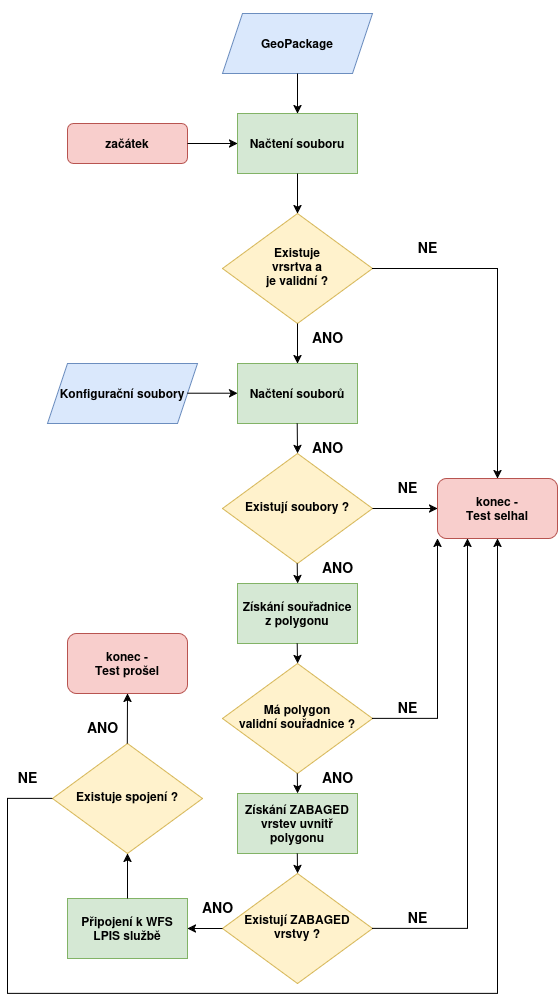
\includegraphics[height=17cm]{pictures/test1.png}
\caption{Vývojový diagram testování stahování dat z WFS služeb}
\label{fig:test1}
\end{figure}

\subsection{Testování editace vrstev} \label{test_edit}
\hspace{10mm} Při testu editování vrstev jsou využity tři vstupní vrstvy. Jedna slouží ke kontrole přiřazení kódu využití území z jejího názvu, ta druhá k přiřazení kódu využití území z jejího řídícího atributu a třetí vrstva slouží ke kontrole aplikace bufferu. Pro tyto aplikace také existují tři konfigurační soubory vytvořené speciálně pro ně, které syntaxí mimikují potřebné konfigurační soubory.

\hspace{10mm} K těmto souborům také existují tři korespondující referenční soubory, které slouží pro porovnání výsledků procesů editace vrstev. Existence všech souborů a validita z nich získaných vektorových vrstev v paměti počítače jsou ověřeny.

\hspace{10mm} Pomocí konfiguračních souborů jsou všechny tři vstupní vektorové vrstvy upraveny a po těchto úpravách jsou porovnány s vrstvami referenčními. 

\begin{figure}[H] \label{obr19}
\centering
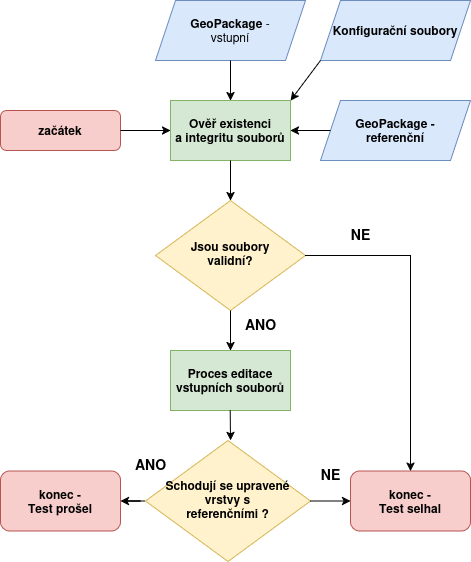
\includegraphics[height=10cm]{pictures/test2.png}
\caption{Vývojový diagram testování editace vrstev}
\label{fig:test2}
\end{figure}


\subsection{Testování získávání dat hydrologických skupin půd} \label{test_soil}
\hspace{10mm} Pro tento test je nutné z konfiguračních souborů načíst URL adresu WPS služby, která zprostředkovává data HSP, a identifikátor pro tuto službu. Dále je potřeba načíst vzor XML dotazu pro tuto službu a polygon, který slouží pro definici zájmového území a je také nutným vstupem WPS služby.

\hspace{10mm} Z polygonu na vstupu jsou získány souřadnice jeho ohrazujícího obdélníku a s dalšími informacemi jsou vloženy do vzorového XML. S WPS službou je následně navázáno spojení.

\hspace{10mm} WPS služba vrací rastr formátu TIF v komprimovaném adresáři. Složka je dekomprimována a rastr je načten do paměti počítače.

\hspace{10mm} Následně je načten do paměti i referenční rastr a pomocí knihovny GDAL jsou porovnány hodnoty jejich pixelů.

\begin{figure}[H] \label{obr20}
\centering
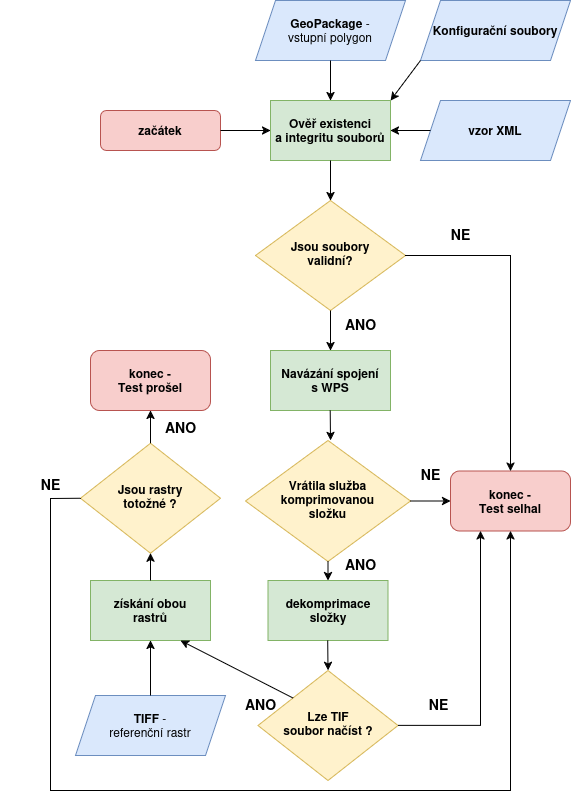
\includegraphics[height=14cm]{pictures/test3.png}
\caption{Vývojový diagram testování stahování dat HSP}
\label{fig:test3}
\end{figure}

\subsection{Testování přiřazení CN hodnot} \label{test_CN}

\hspace{10mm} Pro tento test existuje GeoPackage soubor s potřebnými atributy pro získání CN hodnoty (kód využití území, hydrologická skupina půdy). Také je využita kopie CN tabulky z konfiguračních souborů, aby případná úprava tohoto souboru uživatelem neovlivnila jeho výsledek.

\hspace{10mm} Existence obou souborů a validita vektorové vrstvy jsou ověřeny. Vektorové vrstvě jsou přiřazeny atributy \textit{CN2} a \textit{CN3}. Následně je výsledek porovnán s referenční vektorovou vrstvou získanou z jiného GeoPackage souboru.

\begin{figure}[H] \label{obr21}
\centering
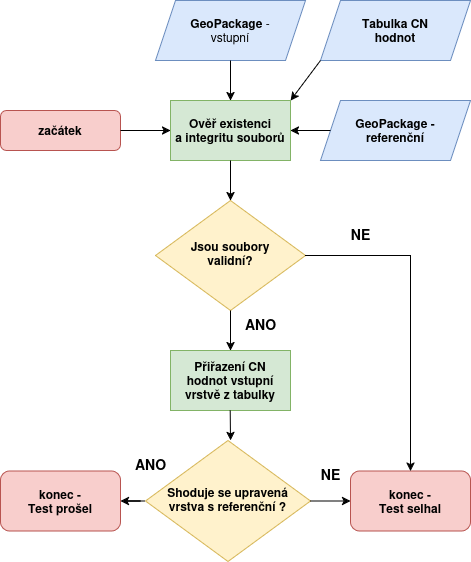
\includegraphics[height=10cm]{pictures/tst4.png}
\caption{Vývojový diagram testování přiřazení CN hodnot}
\label{fig:test4}
\end{figure}


\subsection{Testování získávání vrstev objemů přímých odtoků} \label{test_runoff}
\hspace{10mm} Zde se nejprve ověří správnost vzorců zprostředkovávající hodnoty efektivních srážkových výšek a z nich vypočtených objemů. Na vstup jsou vloženy fiktivní čísla, které jsou po dosazení a výpočtu porovnány s očekávanými čísly.

\hspace{10mm} Další testovanou funkcí je získávání hodnot z CSV souborů. Jednoduchý CSV soubor na vstupu není načítán, ale automatizovaně vytvářen v dočasné složce. Čísla z něj jsou potom načteny funkcí používanou při výpočtu objemů přímých odtoků pomocí WPS služby a porovnány s hodnotami, z nichž byl dočasný soubor vytvořen.

\hspace{10mm} Dále je testována funkce získávající všechny výšky úhrnů srážek v různých dobách opakování. Opět je vytvořen fiktivní CSV soubor s hodnotami ve stejném formátu, který poskytuje WPS služba. Tato funkce vrací, na rozdíl od té předchozí, místo jednotlivých hodnot celý seznam z polí CSV souboru označených dobami opakování, které jsou funkci poskytnuty na vstupu.

\hspace{10mm} Naposledy je testována funkce tvořící atributy vrstvy dle uživatelského vstupu. Testu je poskytnut opět GeoPackage soubor(stejný jako v kapitole \textit{5.9.2}), a tomu jsou přiřazeny atributová pole, dle mimikovaného uživatelského vstupu. Existence nově vytvořených atributových polí je ověřena.

\begin{figure}[H] \label{obr22}
\centering
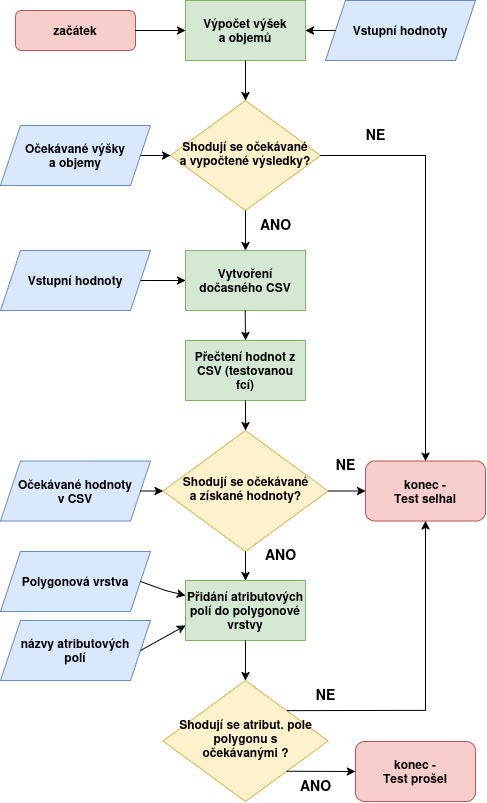
\includegraphics[height=14cm]{pictures/test5.png}
\caption{Vývojový diagram testování při získávání objemů přímých odtoků}
\label{fig:test5}
\end{figure}

\section{Tvorba dokumentace} \label{docs}

\hspace{10mm} Dokumentace je k zásuvnému modulu vyhotovena pomocí MkDocs s využitím šablony 
Material for MkDocs. Pro jednotlivé části jsou vytvořeny Markdown soubory. Na úvodní stránce si uživatel vybere, zda chce dokumentaci zobrazit v české či anglickém jazyce. V dokumentaci je popsán postup instalace, ovládání zásuvného modulu, popis atributových tabulek generovaných vrstev, popis konfiguračních souborů a postupy generování symbologií.

\hspace{10mm} V konfiguračních souborech MkDocs je nastavena hlavní barva prostředí, přepínání tmavého a světlého režimu zobrazení stránky, přepínač jazyka, ikona s odkazem na GitHub repozitář a zápatí stránky s přepínačem vedoucím na předchozí a nadcházející kapitolu.

\begin{figure}[H] \label{obr23}
\centering
\includegraphics[height=7cm]{pictures/docs.png}
\caption{Ukázka úvodní stránky české části dokumentace}
\label{fig:docs}
\end{figure}

\hspace{10mm} Pomocí GitHub Actions jsou z konfiguračních a Markdown souborů generovány HTML stránky při každé úpravě hlavní větve GitHub repozitáře. Generované soubory jsou vždy vloženy do dedikované větve \textit{gh-pages} a z ní jsou publikovány na web pomocí služby GitHub Pages. Odkaz s dokumentací byl vložen do README souboru repozitáře a také byl propojen s tlačítkem v uživatelském rozhraní zásuvného modulu, které po kliknutí otevře okno ve výchozím prohlížeči.

\chapter*{Diskuze} \label{discusion}
\addcontentsline{toc}{chapter}{Diskuze}
\hspace{10mm} V České republice je metoda SCS-CN hojně využívána pro výpočet úhrnu efektivní srážky. Není tedy divu, že existuje řada nástrojů, která v současnosti toto úsilí ulehčuje. Mezi takové patří například softwary HEC-HMS, Atlas HYDROLOGIE, HydroRAIN nebo komerční DesQ-Max-Q. \cite{MNYDGwleJOjKLRU2}

\hspace{10mm} Na rozdíl od těchto nástrojů umožňuje vyvinutý zásuvný modul tvořit vrstvu využití území z aktuálních otevřených dat ZABAGED a LPIS, což považuji za jeho největší přínos. 

\hspace{10mm} I díky tomu by se výsledek této práce dal zařadit mezi QGIS zásuvné moduly sloužící na poli hydrologie, jakými jsou také SMODERP2D \cite{Kavka2024}, což je fyzikálně orientovaný model, který na základě hydrologické bilance a výpočtu proudění povrchového odtoku určuje míru erozního ohrožení.

\hspace{10mm} Mezi zahraniční QGIS zásuvné moduly s podobnou funkcí patří například řecký GWAT \cite{lymperis2024} nebo americký plugin \cite{siddiqui2020} popsán v části této práce 2.1 . Nicméně ty pro určení informací o využití území používají pouze neaktualizovaná rastrová data jako je Corine Land Cover s velikostmi pixelů v řádu desítek metrů.

\hspace{10mm} Generace vrstvy využití území z dat ZABAGED a LPIS má určitě potenciál být rozšířena o přiřazení kódu využití území a bufferu dle více hodnot než jednoho atributového pole, což by mohlo například u kategorizované lesní plochy mohlo znamenat kombinovat informace o výškové i druhové kategorii zároveň. Tato vrstva by také mohla být obohacena o další česká otevřená data jako RUIAN nebo DTM.

\hspace{10mm} Dále by bylo možné detekovat, jaké prvky se nacházejí v intravilánu nebo extravilánu obcí, což může mít u některých vliv na zpřesnění určení využití území.

\hspace{10mm} Využití YAML formátu u konfiguračních souborů přispívá k uživatelsky přívětivé úpravě, nicméně by určitě nebylo na škodu implementovat jejich editaci zprostředkovaně skrz uživatelské rozhraní. K zjednodušení jakýchkoliv úprav jak samotných tvořených vrstev či právě konfiguračních souborů slouží dokumentace.

\hspace{10mm} Stažení vrstev LPIS a ZABAGED s jejich následnou editací může v složitějších územích trvat okolo tří minut. Nicméně je nutno zmínit, že třetinu tohoto času trvá navrácení pouze jediné LPIS vrstvy z WFS služby. Celý tento postup je jako většina dalších přesunuta do vedlejšího vlákna QGIS pro zachování responsivity softwaru. 

\hspace{10mm} Pro zjednodušení instalace by také bylo vhodné v budoucnu zásuvný modul publikovat v oficiálním QGIS repozitáři. Po tomto kroku by již nebylo modul nutné instalovat ze ZIP archivu, ale přímo ze správce zásuvných modulů v QGIS.

\chapter*{Závěr} \label{results}
\addcontentsline{toc}{chapter}{Závěr}
\hspace{10mm} Výsledkem práce je zásuvný modul softwaru QGIS, který umožňuje automatizované stahování českých geodat, jejich ohodnocení atributy a vzájemné propojení. Dle zvolené tabulky umožňuje přiřazení CN hodnot a takovou vrstvu použít jako vstup do výpočtu objemu přímého odtoku pro projektované výšky úhrnů získaných buď uživatelskou definicí nebo pomocí WPS služby pro vybrané doby opakování.

\hspace{10mm} Uživateli je umožněno pro hydrologické analýzy pomocí konfiguračních souborů editovat, jaké vrstvy budou využity pro vytvoření vrstvy využití území a v jakém pořadí budou spojeny. Také je možné definovat prvkům vlastní šířky bufferu či zpřesnění kódu využití území dle hodnoty jejího vybraného atributu. Je také možné definovat uživatelskou tabulku pro získání CN hodnot či jednoduše změnit URL adresy poskytovatelů dat v případě jejich změny.

\hspace{10mm} Uživatelské vstupy jsou před každým procesem kontrolovány, zda splňují potřebné parametry a zásuvný modul je také doplněn o softwarové testy a dokumentaci, která je, včetně odkazu na GitHub repozitář, uvedena jako příloha této práce. Každá vytvořená vrstva má také vlastní definovanou symbologii uchovávanou v barevných tabulkách nebo automaticky přiřazenou.

\hspace{10mm} Zásuvný modul poskytuje výsledky s velkou mírou automatizace nicméně je vhodné, aby byl využíván odborně způsobilými osobami s uvážením vhodnosti základně zvolených parametrů této generace a samotných výsledků. Tomuto je uzpůsobena i volená symbologie zvýrazňující prvky s chybějícími či nevhodnými hodnotami.

\hspace{10mm} Zásuvný modul je publikován pod licencí \textit{GNU General Public License verze 3}, která je převzata z využití QGIS Python API (\textit{PyQGIS}).

\hspace{10mm} Jako možná rozšíření zásuvného modulu bych uvedl například filtrování symbologie tak, aby se zobrazovaly pouze třídy přítomné v aktuální vrstvě, nebo doplnění konfiguračních souborů o buffery a kódy využití území pro více ZABAGED prvků. Jakékoliv další zjištěné nedostatky je možné zmínit v GitHub repozitáři v záložce \textit{"Issues"}.

\hspace{10mm} Dle mého názoru byly stanovené cíle práce celkově splněny a další vývoj bude probíhat na pracovištích Katedry geomatiky \textit{(K155)} a Katedry hydromeliorací a krajinného inženýrství \textit{(K143)}.


\clearpage  % SEM NESAHEJTE!
\addcontentsline{toc}{chapter}{Seznam použité literatury}  \label{zdroje}

\begin{thebibliography}{1}
\bibitem{MNYDGwleJOjKLRUp}
PONCE, V. M. and HAWKINS R. H. 1996. Runoff curve number: Has it reached maturity?
\textit{ Journal of Hydrologic Engineering 1(1):11-19. Dostupné z: \href{https://ponce.sdsu.edu/runoff11view.html}
{https://ponce.sdsu.edu/runoff11view.html}}

\bibitem{Holman2003}
HOLMAN, I.P.; HOLLIS, J.M.; BAMLEY, M.E. a THOMPSON, T.R.E. The contribution of soil structural degradation to catchment flooding: a preliminary investigation of the 2000 floods in England and Wales. \textit{Hydrology and earth system sciences}. 2003, roč. 7, č. 5, s.~754-765.

\bibitem{Lian2020}
LIAN, Huishu; YEN, Haw; HUANG, Jr-Chuan; FENG, Qingyu; QIN, Lihuan et al. CN-China: Revised runoff curve number by using rainfall-runoff events data in China. \textit{Water Research}. 2020, roč. 2020, č. 177, s.~115767. ISSN 0043-1354. Dostupné také z: \url{https://www.sciencedirect.com/science/article/pii/S0043135420303043}.

\bibitem{MNYDGwleJOjKdRUp}
PODHRÁZSKÁ, Jana; BEDNÁŘ, Marek; DOSTÁL, Tomáš; DUMBROVSKÝ, Miroslav; HANEL, Martin et al. \textit{Ochrana zemědělské půdy před erozí: metodika}. Praha: Výzkumný ústav meliorací a ochrany půdy, 2024. ISBN 978-80-7212-667-5.

\bibitem{MNYDGwleJOjKLRU2}
KAVKA, Petr a KAŠPAR, Marek. Krátkodobé srážky pro hydrologické modelování a navrhování drobných vodohospodářských staveb v krajině: Certifikovaná metodika.
\textit{ Fakulta stavební ČVUT v Praze, 2023. ISBN 978-80-01-07115-1}

\bibitem{MNYDGwleJOjKLRU3}
JANEČEK, M. a P. KOVÁŘ. Aktuálnost „Metody čísel odtokových křivek –
CN“ k určování přímého odtoku z malého povodí.
\textit{ Vodní hospodářství. 2010,
č. 7, s. 187-189.} 

\bibitem{MNYDGwleJOjKLRU5}
Urban hydrology for small watersheds: Technical Release 55 (TR-55) (Second ed.).
\textit{ Natural Resources Conservation Service. Conservation Engineering Division, 1986.}

\bibitem{Kulasova2004}
KULASOVÁ, B.; ŠERCL, P. a BOHÁČ, M. \textit{Verifikace metod odvození hydrologických podkladů pro posuzování bezpečnosti vodních děl za povodní: závěrečná zpráva projektu QD1368}. ČHMÚ Praha, 2004.



\bibitem{dile2016}
Dile, Yihun Taddele, Louise Karlberg, Raghavan Srinivasan, and Johan Rockström. 
\newblock Investigation of the Curve Number Method for Surface Runoff Estimation in Tropical Regions. 
\newblock \emph{Journal of the American Water Resources Association (JAWRA)}, 2016, pages 1--15. 
\newblock DOI: \href{https://doi.org/10.1111/1752-1688.12446}{10.1111/1752-1688.12446}.

\bibitem{Batvari2021}
BATVARI, B. Prabhu Dass a NAGAMANI, K. GIS-Based Surface Runoff Modeling Using Empirical Technique For A River Basin In South India. Online. \textit{Nature Environment and Pollution Technology An International Quarterly Scientific Journal}. 2021, vol.~20, no. 5, s.~2117-2123. ISSN 2395-3454. Dostupné z: \url{https://doi.org/10.46488/NEPT.2021.v20i05.029}. [cit. 2025-04-17].


\bibitem{dONaeOjXanl1W2md}
ČSN P ISO/TS 19104, \textit{Geografická informace - Terminologie}. 2010.

\bibitem{Matejova2019}
MATEJOVÁ, Vlasta. \textit{Quantum GIS}. Diplomová práce. České Budějovice: Jihočeská univerzita v Českých Budějovicích, Ekonomická fakulta, 2019.

\bibitem{Baghdadi2018}
BAGHDADI, Nicolas; MALLET, Clément a ZRIBI, Mehrez. \textit{QGIS and Generic Tools}. Volume 1. John Wiley \& Sons, 2018. ISBN 9781119457091.

\bibitem{QPwvEntkWdxPk0Lz}
QGIS DEVELOPMENT TEAM. \textit{QGIS geographic information system}. Online. 2025. Dostupné z: \url{https://www.qgis.org}. [cit. 2025-01-26].

\bibitem{siddiqui2020}
Siddiqui, Abdul Raheem. \textit{Curve Number Generator: A QGIS Plugin to Generate Curve Number Layer from Land Use and Soil}. 2020. [cit. 2025-04-17]. Available at: \url{https://github.com/ar-siddiqui/curve_number_generator}.

\bibitem{nEFEg7XpI9hVQCiO}
\textit{Katalog objektů ZABAGED®}. Verze 4.4. Zeměměřický úřad, 2024.


\bibitem{Devaty2018}
DEVÁTÝ, Jan. \textit{Klasifikace území pro erozní modely pomocí GIS a veřejně dostupných datových zdrojů}. Disertační práce. Praha: České vysoké učení technické v Praze, Fakulta stavební, Katedra hydromeliorací a krajinného inženýrství, 2018.

\bibitem{KocurBera2019}
KOCUR-BERA, Katarzyna. Data compatibility between the Land and Building Cadaster (LBC) and the Land Parcel Identification System (LPIS) in the context of area-based payments: A case study in the Polish Region of Warmia and Mazury. \textit{Land Use Policy}. 2019, roč. 2019, č. 80, s.~370-379. ISSN 0264-8377.

\bibitem{sSYEwLE0rNKoWGYk}
\textit{Nařízení vlády č. 307/2014 Sb. o stanovení podrobností evidence využití půdy podle uživatelských vztahů}. 2014. Dostupné také z: \url{http://www.zakonyprolidi.cz/cs/2014-307}.

\bibitem{Strouhal2022}
STROUHAL, Luděk a KAVKA, Petr. Hydrologické skupiny půd --- rozevřené nůžky hydrologických výpočtů (2. část). \textit{Vodní hospodářství}. 2022, roč. 72, č. 9, s.~7-12.

\bibitem{Vretanos2014}
VRETANOS, Panagiotis (Peter) A. \textit{OpenGIS Web Feature Service 2.0 Interface Standard --- With Corrigendum}. 2.0.2. Open Geospatial Consortium, 2014.

\bibitem{Zhang2005}
ZHANG, Chuanrong a LI, Weidong. The Roles of Web Feature and Web Map Services in Real-time Geospatial Data Sharing for Time-critical Applications. Online. \textit{Cartography and Geographic Information Science}. 2005, roč. 32, č. 4, s.~269-283. ISSN 1523-0406. Dostupné z: \url{https://doi.org/10.1559/152304005775194728}. [cit. 2025-02-25].

\bibitem{Schall2009}  
SCHALL, Gerhard, MENDEZ, Erick, KRUIJFF, Ernst, VEAS, Eduardo, JUNGHANNS, Sebastian, REITINGER, Bernhard a SCHMALSTIEG, Dieter.  
Handheld Augmented Reality for underground infrastructure visualization.  
\textit{Personal and Ubiquitous Computing}, 2009, roč. 13, s. 281-291.  
DOI: 10.1007/s00779-008-0204-5.  

\bibitem{Stollberg2007}
STOLLBERG, Beate a ZIPF, Alexander. OGC Web Processing Service Interface for Web Service Orchestration Aggregating Geo-processing Services in a Bomb Threat Scenario. In: J. WARE, Mark, E. TAYLOR, George (ed.). \textit{Web and Wireless Geographical Information Systems}. Anglie, Cardiff: Springer, 2007, s.~239-251. ISBN 978-3-540-76923-1.

\bibitem{5Xjhvf3W3tsG6nhX}
\textit{OGC® WPS 2.0.2 Interface Standard Corrigendum 2}. 2.0.2. Open Geospatial Consortium, 2015.

\bibitem{hsOq0virmVAO85Ud}
BEN-KIKI, Oren; EVANS, Clark a DÖT NET, Ingy. \textit{YAML Ain-t Markup Language (YAML) Version 1.2}. 3rd Edition, Patched at 2009-10-01.

\bibitem{Summerfield2007}
SUMMERFIELD, Mark. \textit{Rapid GUI Programming with Python and Qt: The Definitive Guide to PyQt Programming}. Pearson Education, 2007. ISBN 978-0132703062.

\bibitem{Okken2017}
OKKEN, Brian. \textit{Python Testing with pytest: Simple, Rapid, Effective, and Scalable}. Pragmatic Bookshelf, 2017. ISBN 9781680502404.

\bibitem{Guthals2023}
GUTHALS, Sarah. \textit{GitHub\texorpdfstring{\textsuperscript{\textregistered}}{ (R)} For Dummies \texorpdfstring{\textsuperscript{\textregistered}}{(R)}}. 2nd Edition. Hoboken, New Jersey: John Wiley \& Sons, 2023. ISBN 978-1-394-15917-8.

\bibitem{Cone2020}
CONE, Matt. \textit{The Markdown Guide}. Matt Cone, 2020. ISBN 979-8656504492.

\bibitem{Christie2014}
CHRISTIE, Tom. \textit{MkDocs Team}. Online. MkDocs.~2014. Dostupné z: \url{https://www.mkdocs.org/}. [cit. 2025-05-06].

\bibitem{Kavka2024}
KAVKA, Petr; LANDA, Martin; JEŘÁBEK, Jakub; PEŠEK, Ondřej. \textit{SMODERP – Distributed event-based model for surface and subsurface runoff and erosion}, version 2.0.1. Sep. 2024. [cit. 2025-05-12]. Dostupné z: \url{https://github.com/storm-fsv-cvut/smoderp2d}.

\bibitem{lymperis2024}
LYMPERIS, Efstathios. \textit{GWAT – Watershed Analysis Toolbox}, version 3.0.0. 11 Nov. 2024. [cit. 2025-05-12]. Dostupné z: \url{https://plugins.qgis.org/plugins/gwat/}.


\end{thebibliography}

\label{list_pics}
\addcontentsline{toc}{chapter}{Seznam obrázků}  
\listoffigures

\label{list_tables}
\addcontentsline{toc}{chapter}{Seznam tabulek}  
\listoftables
\chapter*{Seznam ukázek kódu} \label{list_code}
\addcontentsline{toc}{chapter}{Seznam ukázek kódu}  

\begin{itemize}
\item \hyperref[kod:md]{Kód 1.1: Ukázka Markdown syntaxe} \dotfill 23
\item \hyperref[kod:extent]{Pseudokód 2.1: Získání územního rozsahu} \dotfill 29
\item \hyperref[kod:wfs]{Pseudokód 2.2: Stažení vrstvy z WFS služby} \dotfill 30
\item \hyperref[kod:buffer]{Pseudokód 2.3: Přiřazení velikosti bufferu} \dotfill 31
\item \hyperref[kod:extenttoplg]{Kód 2.4: Převod výřezu obrazovky na polygon} \dotfill 32
\item \hyperref[kod:wps]{Kód 2.5: Spuštění komunikace s WPS službou} \dotfill 32
\item \hyperref[kod:polygonizace]{Kód 2.6: Polygonizace rastrové vrstvy} \dotfill 33
\item \hyperref[kod:intersection]{Kód 2.7: Propojení vrstev využití území a HSP} \dotfill 33
\item \hyperref[kod:cncsv]{Kód 2.9: Ukázka layers\_merging\_order.csv} \dotfill 36
\item \hyperref[kod:zabaged_to_LandUseCode_table.yaml]{Kód 2.10: Ukázka zabaged\_to\_LandUseCode\_table.yaml} \dotfill 36
\item \hyperref[kod:ZABAGED.yaml]{Kód 2.11: Ukázka ZABAGED.yaml} \dotfill 37
\item \hyperref[kod:LPIS.yaml]{Kód 2.12: Ukázka LPIS.yaml} \dotfill 38
\item \hyperref[kod:CN_table.csv]{Kód 2.13: Ukázka CN\_table.csv} \dotfill 39
\item \hyperref[kod:CR_check]{Pseudokód 2.14: Ukázka kontroly umístění zájmového území v ČR} \dotfill 40
\item \hyperref[kod:overlap_check]{Pseudokód 2.15: Ukázka kontroly překrytí obou vrstev} \dotfill 41
\item \hyperref[kod:csv_check]{Pseudokód 2.16: Ukázka kontroly CSV souboru} \dotfill 42
\item \hyperref[kod:runoff_check]{Pseudokód 2.17: Ukázka kontroly uživatelského vstupu výšky úhrnu srážky} \dotfill 43


\end{itemize}

\chapter*{Seznam použitých zkratek} \label{list_abr}
\addcontentsline{toc}{chapter}{Seznam použitých zkratek}

\begin{itemize}
  \item API - \textit{application programming interface}, rozhraní pro programování aplikací
  \item CN - \textit{curvature number} - číslo odtokové křivky
  \item CTU - \textit{Czech Technical University} - České vysoké učení technické
  \item CSV - \textit{Comma-Separated Values} - souborový formát
  \item ČHMÚ - Český hydrometeorologický ústav
  \item ČR - Česká republika
  \item ČSN - česká technická norma
  \item DMR - digitální model reliéfu
  \item DMP - digitální model povrchu
  \item DPB - díl půdního bloku
  \item DTM - Digitální technická mapa
  \item ESA - \textit{European Space Agency} - Evropská kosmická agentura
  \item FTP - \textit{File Transfer Protocol} - standardní komunikační protokol
  \item GIS - Geografický informační systém
  \item GML - \textit{Geography Markup Language} - jazyk uchovávající geografické informace
  \item GPL - \textit{General Public License} - softwarová licence 
  \item GNU - \textit{GNU's Not Unix!} - projekt zaměřený na svobodný software
  \item GRID - ZABAGED data nadmořské výšky v síti
  \item HEC-HMS - \textit{Hydrologic Engineering Center -Hydrologic Modeling System },  hydrologický software
  \item HSP - hydrologické skupiny půd
  \item HSG - \textit{Hydrologic Soil Group}, hydrologické skupiny půd
  \item HTML - \textit{Hypertext Markup Language}, značkovací jazyk
  \item INSPIRE - \textit{Infrastructure for Spatial Information in the European Community}, infrastruktura prostorových dat
  
  \item JSON - \textit{JavaScript Object Notation}, formát zápisu dat
  \item LPIS - \textit{Land Parcel Identification System}, systém identifikace pozemků
  \item MIT - \textit{Massachusetts Institute of Technology}, institut stojící za stejnojmennou licencí
  \item NULL - označení prázdné hodnoty
  \item OGC - \textit{Open Geospatial Consortium}, mezinárodní standardizační organizace 
  \item ORNL - \textit{Oak Ridge National Laboratory}, výzkumná instituce
  \item OS - operační systém
  \item OSGeo - \textit{Open Source Geospatial Foundation}, nezisková organizace
  \item PB - půdní blok
  \item PDF - \textit{Portable Document Format}, formát dokumentů
  \item PyQT - python knihovna 
  \item RUIAN - Registr územní identifikace, adres a nemovitostí
  \item SCS-CN - \textit{The Soil Conservation Service - Curve Number}, metoda odtokových křivek
  \item SMODERP - Simulační model povrchového odtoku a erozního procesu
  \item SQL - \textit{Structured Query Language}, standardizovaný strukturovaný dotazovací jazyk
  \item TIN - \textit{ triangulated irregular network }, nepravidelná trojúhelníková síť
  \item TIF - (někdy též TIFF) - \textit{Tagged Image File Format} formát rastrových souborů
  \item URL - \textit{Uniform Resource Locator}, jednotný lokátor zdroje
  \item USA - Spojené státy americké
  \item USDA - \textit{U. S. Department of Agriculture}, Americké ministerstvo zemědělství
  \item VÚMOP - Výzkumný ústav monitoringu a ochrany půdy, v. v. i.
  \item WMS - \textit{Web Map Service}, webová mapová služba
  \item WPS - \textit{Web Processing Service}, webová geoprocessingová služba
  \item WYSIWYG - \textit{What you see is what you get}, intuitivní způsob editace dokumentů v počítači
  \item XML - \textit{Extensible Markup Language}, značkovací jazyk
  \item YAML - \textit{YAML Ain't Markup Language}, jazyk pro serializaci dat
  \item ZABAGED - Základní báze geografických dat
  \item ZM - Základní mapa České republiky 
 \end{itemize}


\chapter*{Seznam příloh} \label{list_attach}
\addcontentsline{toc}{chapter}{Seznam příloh}  

\begin{enumerate}
  \item Odkazy na GitHub repozitář a dokumentaci
  \item Dokumetace zásuvného modulu
\end{enumerate}

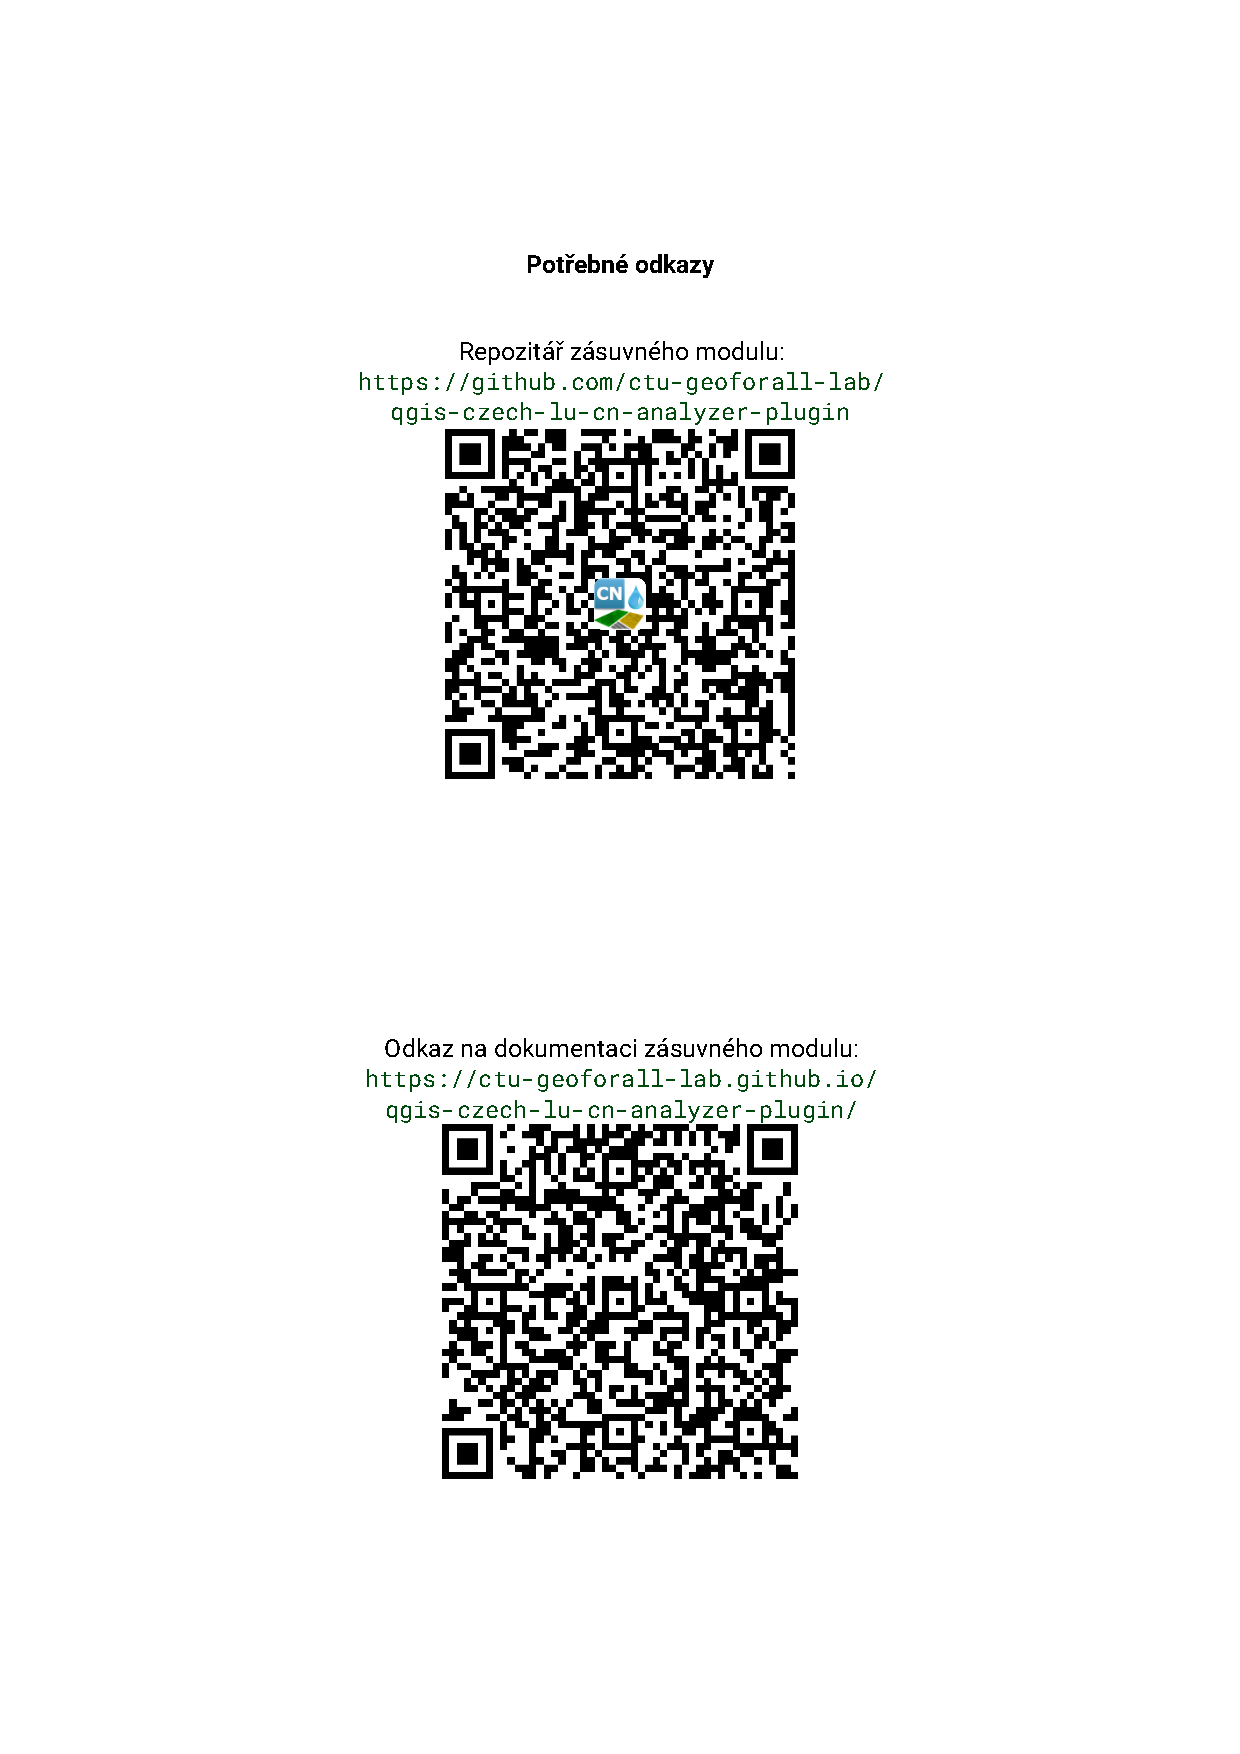
\includepdf[pages={1}]{PRILOHA_A.pdf} 
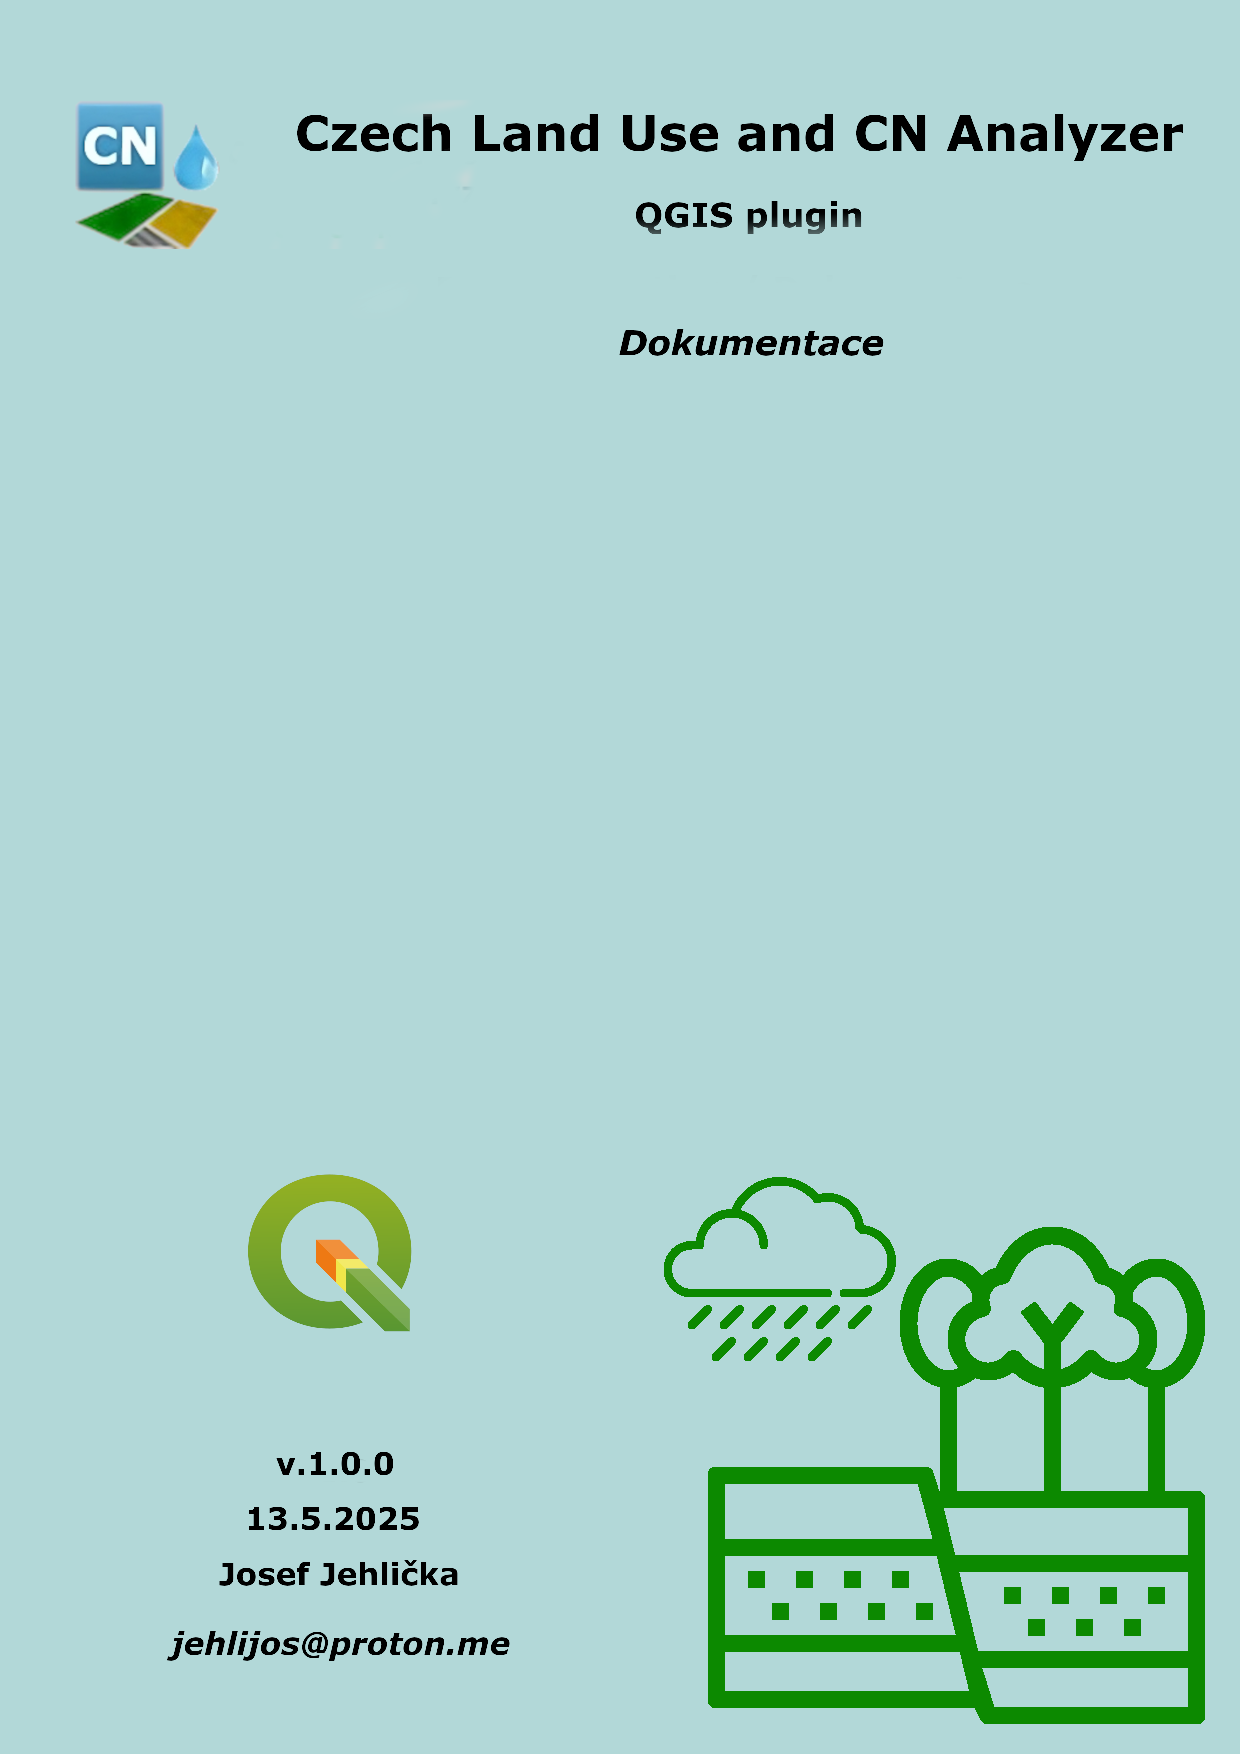
\includepdf[pages=-]{PRILOHA_B.pdf} 
  
\end{document}

